\documentclass[a4paper,12pt,oneside,spanish]{book}
\usepackage[utf8]{inputenc}
\usepackage{babel}
\usepackage{amsmath}
\usepackage[colorlinks]{hyperref}
\usepackage{graphicx}
\usepackage[acronym,toc,xindy]{glossaries}

\newcommand{\grad}{\hspace{-2mm}$\phantom{a}^{\circ}$}


\author{Mariano Gabriel Gili}
\title{Tesis}
\date{\today}

%%%%%%%%%%%%%%%%%%%%%%%%%%%%%
%%% Glosario            %%%%%
%%%%%%%%%%%%%%%%%%%%%%%%%%%%%
\makeglossaries

\newglossaryentry{hola}{name={hola},description={Esto es una prueba}}

%%%%%%%%%%%%%%%%%%%%%%%%%%%%%
%%% Siglas              %%%%%
%%%%%%%%%%%%%%%%%%%%%%%%%%%%%
\newacronym{mde}{MDE}{Ingeniería de Software Dirigida por Modelos o Model-Driven Engineering}
\newacronym{mda}{MDA}{Arquitectura Dirigida por Modelos o Model-Driven Architecture}
\newacronym{omg}{OMG}{Object Management Group}
\newacronym{mdd}{MDD}{Desarrollo Dirigido por Modelos o Model-Driven Development}
\newacronym{ieee}{IEEE}{Institute of Electrical and Electronics Engineers}
\newacronym{ide}{IDE}{Entornos de Desarrollo Integrados o Integrated Development Environment}
\newacronym{uml}{UML}{Unified Modeling Language}
\newacronym{mof}{MOF}{MetaObject Facility}
\newacronym{emf}{EMF}{Eclipse Modeling Framework}
\newacronym{ocl}{OCL}{Object Constraint Language}
\newacronym{evl}{EVL}{Epsilon Validation Language}
\newacronym{teap}{TEAP}{Traceability Elicitation and Analysis Process}
\newacronym{alm}{ALM}{Application Lifecycle Management}
\newacronym{soa}{SOA}{Service Oriented Architecture}
\newacronym{ria}{RIA}{Rich Internet Applications}
\newacronym{rcp}{RCP}{Rich Client Platform}
\newacronym{epl}{EPL}{Eclipse Public License}
\newacronym{api}{API}{Interfaz de programación de aplicaciones o Application Programming Interface}
\newacronym{swt}{SWT}{Standard Widget Toolkit}
\newacronym{xmi}{XMI}{XML Metadata Interchange}
\newacronym{gui}{GUI}{Interfaz de Usuario Gráfica o Graphical User Interface}
\newacronym{jdt}{JDT}{Java Development Tooling}
\newacronym{gmf}{GMF}{Graphical Modeling Framework}
\newacronym{gef}{GEF}{Graphical Editing Framework}
\newacronym{spl}{SPL}{Línea de Producto de Software o Software Product Line}
\newacronym{case}{CASE}{Computer Aided Software Engineering}
\newacronym{qvt}{QVT}{Query/View/Transformation}
\newacronym{dsl}{DSL}{Domain-Specific Language}
\newacronym{atl}{ATL}{Atlas Transformation Language}
\newacronym{mmt}{MMT}{Model-to-Model Transformation}



\begin{document}

%%%%%%%%%%%%%%%%%%%%%%%%%%%%%
%%% Título %%%%
%%%%%%%%%%%%%%%%%%%%%%%%%%%%%
 \maketitle

\frontmatter
%%%%%%%%%%%%%%%%%%%%%%%%%%%%%
%%% Índices %%%%
%%%%%%%%%%%%%%%%%%%%%%%%%%%%%
\tableofcontents
\listoffigures


%%%%%%%%%%%%%%%%%%%%%%%%%%%%%
%%% Agradecimientos %%%
%%%%%%%%%%%%%%%%%%%%%%%%%%%%%
\chapter{Agradecimientos}


Agradezco a todos...  holaaaaaaaa.

puede ser que \gls{hola}


%%%%%%%%%%%%%%%%%%%%%%%%%%%%%
%%% Introducción %%%
%%%%%%%%%%%%%%%%%%%%%%%%%%%%%
\chapter{Introducción}


En la \gls{mde}, se define al modelo como principal artefacto que toma participación a lo largo de todas las tareas/procesos de la ingeniería de software – análisis, diseño, desarrollo, pruebas, mantenimiento, etc. Una implementación particular propuesta que sigue esta idea es la \gls{mda}, definida por el \gls{omg}, cuyo ciclo de proceso de desarrollo está basado enteramente en el uso de modelos formales y transformaciones que se realizan sobre dichos modelos. Una característica muy importante de todo proceso de \gls{mdd}, es lo que se conoce como “posibilidad de rastreo” (o de ahora en más en inglés traceability), que ayuda y toma parte en todo lo que respecta a las relaciones que existen entre cada uno de los artefactos productos del proceso de desarrollo.

Cuando nos referimos al término artefacto, hablamos por ejemplo de un requerimiento de sistema, un componente de software, un caso de prueba, entre otros. El mantenimiento y la definición de las relaciones y dependencias que existen entre los artefactos no es una tarea fácil, el mismo ha sido un desafío desde principios de 1970.

En el presente documento de tesis se abordará el tema de traceability, luego se presentará un análisis de los distintos problemas que aún se encuentran abiertos como así también un conjunto de soluciones encontradas a lo largo de la investigación. Finalmente, se elaborará un esquema de traceability con el fin de contribuir en la solución de alguno de los problemas nombrados.




\chapter{Objetivos}


El objetivo del trabajo de tesis propuesto comprende, por un lado, una introducción al tema de traceability conjunto con un análisis de los problemas que aún se encuentran abiertos en su ámbito en \gls{mde}, seguido de la elaboración de un esquema de traceability que contribuya en la solución de dichos problemas.

También se diseñará e implementará una herramienta que pueda ser integrada a otra de desarrollo \gls{mde}, y asista al desarrollador automatizando el proceso de definición de trazas o links entre elementos de los modelos origen y destino. Esta solución proveerá un mapa de transformaciones que permitirá determinar la procedencia de cada ítem del modelo destino, y su correspondiente origen en el modelo fuente.


\mainmatter
%%%%%%%%%%%%%%%%%%%%%%%%%%%%%
%%% Traceability %%%
%%%%%%%%%%%%%%%%%%%%%%%%%%%%%
\chapter{Traceability}

\section{Introducción}

Según el Glosario Estándar de Términos de la Ingeniería de Software del \gls{ieee} \cite{IEEE} la noción de traceability se define como: El grado o nivel en el cual una relación puede ser establecida entre dos o más productos del proceso de desarrollo, especialmente entre productos que tengan una relación de predecesor-sucesor o principal-secundario; por ejemplo el grado en el cual el requerimiento y el diseño de un componente de software se corresponden. La definición anterior fue dada por “the requirements management community”, para nosotros, que necesitamos un punto de vista maś cercano al contexto de \gls{mdd}, traceability es un término usado para describir cualquiera de las complejas relaciones lógicas que existen entre los distintos artefactos que se presentan en cualquier momento del ciclo de vida del desarrollo de software, el establecimiento de estas relaciones y/o el mantenimiento de las mismas.

Entre varios beneficios de traceability que enumeraremos mejor más adelante, podemos encontrar que ayuda a identificar las relaciones y dependencias que existen entre los artefactos de software. También traceability es crucial entre los requerimientos y su representación en los modelos para asegurar que el conjunto relevante de requerimientos fueron debidamente implementados en el código. Pero no solo traceability asegura la identificación de objetos y elementos relacionados, también puede facilitar el análisis de impactos de cambios durante el desarrollo de software.

Las relaciones de traceability pueden ser definidas de forma automática, por ejemplo producto de una transformación de modelos, o de forma manual como el caso de una relación de implementación entre un requerimiento y un componente de software.

En la ingeniería de software encontramos dos usos o semánticas principales que dependen del contexto de traceability:

\begin{itemize}

\item Traceability en la ingeniería de requerimientos: donde se guarda un requerimiento desde su definición hasta su implementación. En más detalle según \cite{GotelFinkelstein} se refiere a la habilidad de describir y seguir la vida de los requerimientos en ambas direcciones, hacia delante y hacia atrás (forward and backward traceability). Desde los orígenes, pasando por el desarrollo y la especificación, hacia su posterior entrega y uso, y a través de todos los períodos de refinamiento e iteración de cualquiera de estas etapas.

\item Traceability en el Desarrollo Dirigido por Modelos: donde se almacenan principalmente las relaciones existentes entre los artefactos producto de las transformaciones de modelos.

\end{itemize}

\subsection{Beneficios}

A continuación se listan un conjunto de actividades de diferentes dominios de la ingeniería en las cuales el uso de traceability es muy beneficioso según \cite{BrcinaRiebisch} y \cite{GrammelVoigt}:

\begin{itemize}

\item En el Análisis de sistemas: nos ayuda a entender la complejidad de un sistema navegando a lo largo del modelo de enlaces obtenidos por la ejecución de las distintas cadenas de transformación.

\item En el Análisis de cobertura: por ejemplo en el momento de ejecución de los casos de prueba, el uso de traceability es crucial para la hora de determinar si todos los requerimientos fueron cubiertos o tenidos en cuenta.

 \item En el Análisis de impacto de cambios: traceability nos ayuda a ver cómo los cambios en un modelo repercutirán en los otros modelos relacionados; también el uso de traceability nos permite saber en cualquier momento el tipo de dependencia que existe entre las entidades relacionadas, lo cual ayuda a determinar la necesidad de un cambio.

 \item En el Análisis de huérfanos: nos permitirá encontrar fácilmente los elementos huérfanos de un modelo dado que serán los artefactos que no se encuentren enlazados a ninguna traza.

 \item En la Comprensión del software y la ingeniería inversa: crucial cuando sea necesario identificar todas las entidades relacionadas a una en particular, entender el tipo de relación existente, identificar las abstracciones, es decir los patrones de diseño, estilos de arquitectura, principios.

 \item En el análisis de requerimiento: por ejemplo para identificar el artefacto particular que demanda una propiedad específica; encontrar y resolver un conjunto de requerimientos que se contradicen.

 \item Apoyo en la toma de decisiones: para justificar una decisión dado que nos facilita entender qué factores y metas influyen en la misma; también traceability nos será muy útil en los momentos que se nos presenten distintas propuestas de solución en su análisis y evaluación.

\item En la Configuración del sistema y versionado: en este momento el uso de traceability es beneficioso para identificar las restricciones entre los componentes, identificar los cambios necesarios para resolver una restricción, identificar las diferencias entre dos versiones distintas del mismo artefacto y su impacto en otros artefactos.

\end{itemize}


\subsection{Algunos inconvenientes}

Aunque las ventajas de traceability hoy día ya han sido identificadas, su puesta en práctica apenas ha quedado establecida. Las principales razones de lo anterior según \cite{GrammelVoigt} puede ser por lo siguiente:

\begin{itemize}

 \item El alto costo de la creación y mantenimiento manual de la información de traceability.

\item La falta de heurísticas que determinen qué información de los enlaces deben ser grabados.

 \item Discrepancias entre los distintos roles de usuarios de traceability, por ejemplo entre quienes crean los enlaces y quienes los usan.

\item Carencia de soporte adecuado en las herramientas.

\item Los artefactos son escritos en diferentes lenguajes, por ejemplo los requerimientos se escriben en lenguaje natural mientras que los programas en algún lenguaje de programación.

\item Los artefactos describen el sistema de software en diferentes niveles de abstracción, los artefactos usados durante el diseño difiere de los usados en su implementación.

\end{itemize}

Más adelante en otro capítulo se presentará con más detalle los desafíos presentes en la implementación y el uso de traceability.




%%%%%%%%%%%%%%%%%%%%%%%%%%%%%
%%% Problemas y Desafíos %%%
%%%%%%%%%%%%%%%%%%%%%%%%%%%%%
\chapter{Problemas y Desafíos}

En este capítulo vamos a describir los principales problemas y grandes desafíos que se encuentran abiertos en el ámbito de traceability a lo largo de distintos aspectos definidos por \cite{Excellence}.

El capítulo se encuentra organizado principalmente por temas. Luego, para cada tema, se describen sus problemas y a continuación se listan los desafíos que resultan de los mismos:

\section{Sobre el conocimiento de traceability}

\subsubsection{Problemas}

\begin{itemize}

\item[-] Existe poco consenso respecto a cuáles son las mejores técnicas y métodos para la aplicación de traceability, pocas anotaciones y documentación sobre las mejores prácticas, sumado a una falta de recursos que provean una buena base de conocimiento.

\item[-] Las definiciones semánticas no coinciden y las terminologías son dispares o distintas, todo ésto crea barreras de comunicación.

\end{itemize}

\subsubsection{Desafíos}

\begin{itemize}

\item[+] Crear una base de conocimiento en la que se vuelquen las mejores prácticas de traceability, una terminología estándar y mucha información adicional, como por ejemplo casos de estudio.

\end{itemize}

\section{Sobre la capacitación y la certificación}

\subsubsection{Problemas}

\begin{itemize}
\item[-] Muy poca gente es competente en la definición de trazas y, por otro lado, existen disponibles pocos programas educativos.

\item[-] Existen pocos programas de certificación, y de ellos, pocos incluyen componentes de traceability.

\item[-] No hay definido un conjunto estándar de estrategias de traceability.

\end{itemize}

\subsubsection{Desafíos}

\begin{itemize}
\item[+] Identificar las áreas de conocimientos centrales y las habilidades y/o estrategias asociadas a traceability.

\item[+] Desarrollar buenos componentes educativos para la puesta en práctica de traceability.

\item[+] Desarrollar materiales pedagógicos efectivos para educar con énfasis en la importancia y administración de los costos-beneficios del uso de traceability.

\end{itemize}

\section{Sobre el soporte a la evolución}

\subsubsection{Problemas}

\begin{itemize}

\item[-] La información precisa, coherente, completa y actualizada sobre traceability es fundamental para diversos ámbitos y aplicaciones. Sin embargo, las técnicas actuales de “recuperación de trazas” aún son realizadas de forma manual y por lo tanto son propensas a errores.

\item[-] Para que los enlaces de traceability sean útiles, éstos deben reflejar la dependencia actual entre los artefactos. Dado que el costo y esfuerzo para mantenerlos durante la evolución del sistema es inmenso, a menudo los enlaces pasan a encontrarse en un estado erróneo o incorrecto.

 \item[-] Las herramientas actuales de administración de requerimientos incluyen características como “suspect trace links” para ayudar a los analistas a administrar la evolución de los enlaces, pero en la mayoría de los proyectos complejos el número de “suspect trace links” se vuelve rápidamente excesivo, minimizando drásticamente la utilidad de tal característica.
 
\item[-] Los enlaces de traceability tienen que evolucionar de forma sincrónica con los artefactos relacionados, sin embargo los sistemas actuales de gestión de cambios y la semántica de los enlaces no son lo suficientemente sofisticados como para apoyar esta evolución.

\item[-] Los métodos para transformar y reusar los enlaces sincrónicamente con los productos de desarrollo en línea son inmaduros.

\end{itemize}

\subsubsection{Desafíos}

\begin{itemize}

\item[+] Desarrollar técnicas de “recuperación de trazas” para artefactos textuales que sean tan precisos como el proceso manual y a la vez mucho más efectivos en tiempo y costo.

\item[+] Desarrollar la recuperación de trazas para que se encuentren integrados a los \gls{ide}.

\item[+] Desarrollar sistemas de administración de cambios que efectivamente soporten la evolución de los enlaces de trazas sobre múltiples tipos de artefactos.

\item[+] Desarrollar técnicas que soporten traceability en todos los componentes de una línea de productos maximizando la reutilización y la disponibilidad de traceability entre diferentes versiones de los mismos.

\item[+] Desarrollar técnicas para maximizar la reutilización de los enlaces de trazas cuando el código existente se reutiliza en un nuevo producto.

\end{itemize}

\section{Sobre la semántica de los enlaces}

\subsubsection{Problemas}

\begin{itemize}

\item[-] Para efectivamente utilizar los enlaces de trazas y entender las relaciones por debajo de traceability, es necesario definir la semántica de los enlaces, sin embargo definir una formalidad para representar esta semántica no es una tarea fácil y puede llegar a ser acotada a un dominio específico, cosa que no es conveniente.

\item[-] Es muy importante para la consistencia de traceability conocer y establecer la granularidad de los elementos a ser enlazados, pero no existe un modelo claro de costo-beneficio para determinar consistentemente cuál es la granularidad correcta (“trace granularity”).

\end{itemize}

\subsubsection{Desafíos}

\begin{itemize}

\item[+] Definir meta-modelos para representar la información semántica de los enlaces de trazas y proveer ejemplos de instanciación para distintos dominios específicos.

\item[+] Desarrollar técnicas y procesos para determinar la correcta granularidad de los enlaces de trazas en un proyecto.

\end{itemize}

\section{Sobre la escalabilidad}

\subsubsection{Problemas}

\begin{itemize}

\item[-] Las técnicas corrientes de traceability no escalan adecuadamente en proyectos largos.

\item[-] Las herramientas de visualización son esenciales para dar ayuda en la compresión y el uso de la gran cantidad de información de los enlaces de las trazas. Sin embargo, las técnicas de visualización actuales no escalan bien y no son efectivas al presentar información compleja porque carecen de características sofisticadas de filtrado, navegación, consultas, etc.

\item[-] Muchos conjuntos de datos industriales son compuestos por largos e inestructurados documentos que son difíciles de enlazar mediante trazas.
\end{itemize}

\subsubsection{Desafíos}

\begin{itemize}

\item[+] Obtener conjuntos de datos de escala industrial desde varios dominios y usarlos para investigar la escalabilidad de las técnicas disponibles actualmente y, si es necesario, crear nuevas aproximaciones que escalen más eficientemente.

\item[+] Desarrollar mecanismos visuales efectivos para soportar la navegación y consulta de un gran número de enlaces de traceability y sus artefactos asociados.

\item[+] Desarrollar técnicas escalables para marcar las trazas tanto para conjunto de datos heterogéneos y/o grandes y débilmente estructurados.

\end{itemize}


\section{Sobre los factores humanos}

\subsubsection{Problemas}

\begin{itemize}

\item[-] Los métodos automáticos de traceability producen enlaces de trazas candidatos; sin embargo, el proceso es inútil si el analista no es capaz de evaluarlos correctamente para diferenciar los buenos de los malos, o si es incapaz de confiar en la completitud y precisión de los resultados.

\item[-] Idealmente la tarea de encontrar las trazas debería ser invisible durante el proceso de desarrollo, desafortunadamente la generación de trazas y el uso es interrumpido por interacciones humanas porque en los ambientes de desarrollo actuales aún no es posible automatizar todo el proceso.

\item[-] Los enlaces de trazas comunican artefactos semánticamente diferentes, a su vez estos artefactos son creados por diferentes personas y frecuentemente escritos en diferentes documentos. Como resultado, los usuarios de un lado de los enlaces de trazas no entienden bien los artefactos del otro lado de la relación.

\end{itemize}

\subsubsection{Desafíos}

\begin{itemize}

\item[+] Basado en el estudio del uso de herramientas de traceability, crear nuevas herramientas que reúnan las necesidades prácticas que vayan surgiendo.

\item[+] Entender el impacto y las vulnerabilidades de la fallas humanas sobre el proceso de traceability y desarrollar técnicas para ayudar a los analistas a prevenir errores y minimizar el impacto de los mismos cuando ocurran.

\item[+] Desarrollar técnicas para ayudar a los humanos a superar las barreras semánticas del proceso de desarrollo completo.

\end{itemize}

\section{Análisis de costo-beneficio}

\subsubsection{Problemas}

\begin{itemize}

\item[-] En un escenario de traceability completo, los enlaces son creados entre artefactos en un nivel bajo de abstracción, ésto puede ser deseable para propósitos de comprensión, sin embargo este nivel tan bajo no es frecuentemente práctico y efectivo en costo.

\item[-] Existe una carencia de un modelo de costo-beneficio para analizar entre las distintas necesidades de traceability sobre varios proyectos y para diferentes enlaces potenciales dentro de un proyecto.

\end{itemize}

\subsubsection{Desafíos}

\begin{itemize}

\item[+] Definir y desarrollar técnicas efectivas en costo para generar y mantener información de traceability.

\item[+] Definir un modelo de costo práctico para generar y mantener los enlaces de trazas que tomen en consideración factores tales como el tamaño del proyecto, el tiempo, el esfuerzo y la calidad del sistema.

\item[+] Definir un modelo de beneficios para usar enlaces de trazas que tomen en consideración factores como la crítica y la volatilidad, e incorpore el valor logrado mediante el uso de traceability.

\end{itemize}

\section{Sobre los métodos y las herramientas}

\subsubsection{Problemas}

\begin{itemize}

\item[-] Los métodos de recuperación multimedia no son suficientemente sofisticados y soportados, y se ha realizado poco para incorporar tales técnicas multimedia en las herramientas de traceability.

\item[-] Traceability automático es esencial; sin embargo, se hace difícil por la falta de consistencia entre los artefactos, y la imprecisión de los modelos.

\item[-] Traceability implica todas las siguientes actividades: construcción o generación, evaluación, mantenimiento y el uso de los enlaces; sin embargo, no existe una sola herramienta que pueda cubrir todas estas tareas.

\end{itemize}

\subsubsection{Desafíos}

\begin{itemize}

\item[+] Desarrollar métodos efectivos para enlazar artefactos multimedia.

\item[+] Construir métodos y herramientas con altos niveles de automatización para soportar el ciclo de vida entero, que incluya la construcción, la evaluación, el mantenimiento y el uso de los enlaces de trazas.

\item[+] Desarrollar métodos para trazar requerimientos no funcionales.

\end{itemize}

\section{Sobre los procesos}

\subsubsection{Problemas}

\begin{itemize}

\item[-] Traceability no es incluida frecuentemente como una parte integral del ciclo de vida del desarrollo.

\item[-] Traceability automático puede proveer una alternativa efectiva en costo en comparación a la manual, pero la práctica ha mostrado que algunos conjuntos de datos son difíciles de enlazar usando métodos automáticos debido a las inconsistencias en terminología, los estándares, la carencia de estructuras, los formatos heterogéneos, etc.

\end{itemize}

\subsubsection{Desafíos}

\begin{itemize}

\item[+] Construir modelos de proceso que definan el ciclo de vida del marcado de trazas.

\item[+] Desarrollar técnicas para evaluar la habilidad de un conjunto de datos dado para soportar los métodos automáticos de traceability.
 
\end{itemize}

\section{Sobre el cumplimiento}

\subsubsection{Problemas}

\begin{itemize}

\item[-] Los estándares pueden ayudar a asegurar procesos consistentes y completos, aunque abundan los estándares, no está claro si los investigadores o profesionales están enterados de la existencia de los mismos.

\item[-] La comunidad que engloba traceability son eruditos sobre técnicas y procesos de este tema, pero tienen poca influencia sobre los contenidos relacionados a traceability en los procesos estándar de ingeniería de software.

\item[-] No es claro cómo se puede demostrar el cumplimiento de los estándares y regulaciones .

\end{itemize}

\subsubsection{Desafíos}

\begin{itemize}

\item[+] Establecer un mecanismo de comunicación para hacer que la comunidad de expertos de traceability dictamine los estándares relacionados con la tecnología.

\item[+] Lograr una presencia en la comunidad de estándares para influir y/o desarrollar estándares de traceability.

\item[+] Como comunidad, desarrollar y promover escenarios válidos para probar que las herramientas, las técnicas y las metodologías de traceability cumplen con los estándares.

\end{itemize}


\section{Sobre las mediciones y los Benchmarks}

\subsubsection{Problemas}

\begin{itemize}

\item[-] Los estudios empíricos son necesarios para demostrar la eficacia de los métodos de traceability y así, facilitar el trabajo colaborativo y evolutivo entre los investigadores y profesionales, sin embargo, hay una falta de diseños experimentales, metodologías y benchmarks comunes.

\item[-] Las medidas, métodos y métricas propuestas actuales no han sido validadas a través de estudios o pruebas empíricas.

\item[-] No existen o no se han realizado buenas pruebas o “benchmarks” de traceability y/o no son compatibles.

\item[-] No existen pruebas estándares de comparación para aplicar sobre los métodos y técnicas desarrolladas de traceability.

\item[-] La detección de errores en los enlaces de trazas es necesaria para determinar la eficacia del producto y el proceso, sin embargo los modelos de detección de errores actuales aún son primitivos e inválidos.

\end{itemize}

\subsubsection{Desafíos}

\begin{itemize}

\item[+] Definir procesos estándares para la realización de estudios empíricos durante la investigación de traceability.

\item[+] Construir pruebas (benchmarks) para evaluar los métodos y las técnicas de traceability.

\item[+] Definir medidas para evaluar la calidad de los enlaces de trazas tanto forma individual como la de un conjunto.

\item[+] Desarrollar técnicas de evaluación de métodos y procesos de traceability.

\end{itemize}

\section{Sobre la transferencia de tecnología}

\subsubsection{Problemas}

\begin{itemize}

\item[-] El objetivo de la investigación de traceability es la transferencia de soluciones eficaces para la industria, sin embargo en la realidad en la industria son reacios a probar técnicas nuevas donde la eficacia aún no fue demostrada.

\item[-] La carencia de diálogo entre los dos grupos, investigadores y profesionales, limita la accesibilidad de los investigadores a un conjunto de datos reales para testear nuevas técnicas e inhibe la retroalimentación de la industria a los investigadores.

\item[-] Los prototipos de Traceability son generalmente diseñados para mostrar demostraciones de conceptos, sin embargo no son suficientemente rigurosos para el campo de prueba de la industria.

\end{itemize}

\subsubsection{Desafíos}

\begin{itemize}

\item[+] Crear una infraestructura y un conjunto de métodos relacionados para organizar el proceso de transferencia de tecnología.

\item[+] Identificar los casos de estudio exitosos y darle publicidad, para demostrar la efectividad de los costos de las técnicas de traceability en el ámbito industrial.

\item[+] Identificar los usuarios de traceability y definir sus necesidades en términos de calidad, ciclo de vida, comunicación, etc.

\item[+] Incorporar las herramientas de traceability que se encuentren a la vanguardia en los \gls{ide} estándares (tal como Eclipse) y las herramientas de administración de requerimientos industriales.

\end{itemize}



%%%%%%%%%%%%%%%%%%%%%%%%%%%%%
%%% Solución %%%%%
%%%%%%%%%%%%%%%%%%%%%%%%%%%%%
\chapter{Caminando hacia la propuesta}

A continuación se presenta una pequeña introducción a un conjunto de temas que se tuvieron en cuenta a la hora de definir el esquema de traceability propuesto que se presenta en el capítulo \ref{cap:Propuesta}.

\section{Generación de trazas}

Uno de los desafíos presentados en \cite{GrammelVoigt} trata sobre cuál de los dos enfoques de generación de trazas que existen durante una transformación, implícita o explícita, es conveniente utilizar. En la generación implícita la transformación provee un soporte integral de traceability, en cambio en la explícita, queda en manos del desarrollador codificar las reglas de traceability como un modelo más de salida.

A continuación se detallan las ventajas y desventajas de cada enfoque:

\subsection{Implícita}

\paragraph{Ventajas}

\begin{enumerate}

\item La mayor ventaja de la generación de trazas implícita es que no es necesario ningún esfuerzo adicional para obtener los enlaces de trazas entre los modelos de entrada y salida, dado que son generados en paralelo automáticamente con el modelo actual de la transformación.

\end{enumerate}

\paragraph{Desventajas}

\begin{enumerate}

\item El meta-modelo de traceability es fijo: como la mayoría de los enfoques de transformación tienen diferentes meta-modelos, lograr estandarizar entre estos diferentes enfoques es muy complejo.

\item Poca flexibilidad para controlar los datos de traceability, ésto incluye:

\begin{enumerate}

\item El tipo de información guardada: cuando se trazan todos los elementos del modelo referenciado, el número de enlaces puede volverse incomprensible y por lo tanto menos útil. También al presentarse un modelo de transformación grande y complejo puede acarrear un problema en lo que respecta a rendimiento.

\item El nivel de granularidad de la información de traceability: (esto es por ejemplo realizar trazas solo a nivel de archivo o bajar a nivel del contenido del mismo) esta configuración de los enlaces varía de un escenario de traceability a otro.

\item Contexto de la información: por ejemplo por necesidades de un cliente que presente motivos de seguridad, puede requerir que no toda la información de un modelo tiene permitido ser trazada.

\end{enumerate}

\end{enumerate}


\subsection{Explícita}

\paragraph{Ventajas}

\begin{enumerate}

\item Es posible lidiar con traceability como un modelo regular de salida de la transformación e incorporar reglas de transformación adicionales para generarlo. La elección del meta-modelo es entonces completa del programador y no depende del motor de transformaciones. Por lo tanto, la granulación de los enlaces es adaptable.

\end{enumerate}

\paragraph{Desventajas}

\begin{enumerate}

\item Se requiere un esfuerzo adicional para agregar reglas de transformación específicas para traceability, que pueden en consecuencia contaminar la implementación.

\item Como esta tarea es por lo general manual, es propensa a errores y consume mucho tiempo, más aun si pensamos que esta tarea se tiene que repetir para cada transformación que se realice.

\end{enumerate}

\section{Tipos de enlaces}

Otro de los desafíos refiere a la semántica de los enlaces, es necesario frecuentemente distinguir entre los distintos tipos de enlaces que se pueden presentar. Por ejemplo un enlace entre un requerimiento textual y un elemento de modelo, tiene una semántica distinta que una relación de refinamiento dentro de un modelo.

Los tipos de enlaces requeridos por lo general son fuertemente dependientes al proyecto. Por lo cual definir fijamente los tipos de enlaces semánticos tiene la consecuencia de menor flexibilidad para los enlaces que desee trazar el usuario, los cuales serán definidos por las necesidades del proyecto o la compañía.

Es importante remarcar que la determinación de la semántica de un enlace es guiada por la razón del usuario sobre qué quiere realizar o representar con dicho enlace. No predefinir la semántica correctamente de un enlace puede resultar en fallas de razonamientos.

\section{Estrategias de almacenamiento}

Según \cite{DrivalosPaigeFernandesKolovos} hay dos tipos principales de estrategias para almacenar y administrar la información de traceability. En la primera, la información de traceability se encuentra embebida en los modelos a los que ella refiere. En cambio en la segunda, dicha información se encuentra almacenada de forma separada de los modelos:

\subsection{Almacenamiento de enlaces Intra-Modelo}

Como ya se dijo, bajo esta estrategia la información de traceability es almacenada dentro de los artefactos a los que refiere, esto puede ser mediante elementos del modelo o mediante atributos de los elementos del modelo (como etiquetas o propiedades).

Es una estrategia sencilla y amigable, pero puede ser muy problemática por varias razones. Si los enlaces son dirigidos y almacenados solamente en el modelo origen, éstos no son visibles en el modelo destino, a la inversa (almacenados en el destino) nos encontramos con el mismo problema pero en el origen. Por otro lado, si la información de traceability es almacenada en ambos modelos, entonces nos encontramos con el problema de que dicha información se mantenga consistente por cada vez que se realice un cambio.

A todo lo anterior se suma el problema de la polución que se genera en el modelo con la información de traceability que es ajena a su contexto o fin original, dicha polución puede lograr que el modelo se vuelva muy difícil de comprender y mantener.

Por otro lado, en un entorno \gls{mde} es común que los modelos tengan sus propias representaciones y semánticas, lo cual puede volver más complejo diferenciar la información de traceability de los objetos que representan el modelo del dominio.

Como resultado a los inconvenientes anteriores, el análisis automatizado de la información de traceability se hace muy difícil. Los enfoques principales que hacen uso de esta estrategia utilizan construcciones de lenguajes específicas, por ejemplo determinados tipos de enlaces de traceability están representados en los diagramas \gls{uml} mediante el uso de las estereotipos como <<refines>>.

\subsection{Almacenamiento externo de los enlaces}

En esta estrategia la información de traceability se encuentra almacenada de forma separada a los modelos a los que refiere, esto es en un modelo aparte. Esta propuesta tiene dos claras ventajas, la primera es que los modelos origen y destino se mantienen totalmente limpios, con lo cual la polución nombrada en el almacenamiento intra-modelo no sucede. Y la segunda, dado que el modelo en donde se almacena los traceability links se encuentra definido por un meta-modelo con una clara semántica, logra que el proceso de análisis de la información sea mucho más fácil que en la otra estrategia.

Un requisito previo para el almacenamiento externo de los enlaces de traceability, es que los diferentes elementos del modelo tengan identificadores únicos, de modo que las trazas que los relacionan se pueden resolver inequívocamente. Un ejemplo es el mecanismo propuesto por \gls{mof} y por \gls{emf} en la forma de un identificador xmi.id .

\section{Meta-modelos}

Los modelos que determinan los enlaces de traceability se encuentran definidos cada uno por un meta-modelo, éste puede ser clasificado como un “meta-modelo de traceability de propósito general” o un “meta-modelo de traceability de caso específico”.

\subsection{Meta-modelo de propósito general}

En este caso, nos encontramos con un meta-modelo genérico que permite la captura de las relaciones entre cualquier tipo de elementos de modelo. En este meta-modelo, un enlace de traceability se puede conectar con cualquier número de elementos, de cualquier tipo y de cualquier modelo. Las principales ventajas de este tipo de meta-modelo de propósito general son la simplicidad y la uniformidad (dado que todos los modelos conforman el mismo meta-modelo) con lo cual se mejora la interoperabilidad de las herramientas con capacidades de importar, exportar y gestionar traceability en un formato común.

Por otro lado, como el meta-modelo de propósito general no capta casos específicos de enlaces de trazas fuertemente tipados, o sea con semántica y restricciones definidas rigurosamente, se abre la puerta a establecimientos de enlaces ilegítimos. Como por ejemplo en el caso que se quiera representar trazas entre un diagrama de clases y un modelo de base de datos relacional, sabemos que existen vínculos entre las clases del primer modelo y las tablas del segundo, un meta-modelo de traceability genérico permite el establecimiento de enlaces ilegítimos tales como una clase relacionada con una columna.

La provisión de mecanismos de extensión junto con el meta-modelo de propósito general es un método de uso frecuente para permitir un mejor apoyo para el caso de los requisitos específicos. Sin embargo, todavía carecen de la eficacia de los meta-modelos de casos específicos para capturar estos tipos de casos que requieren tal legitimidad entre la información y su semántica.

\subsection{Meta-modelo de caso específico}

En este caso, para cada escenario de traceability se define un meta-modelo específico. Este meta-modelo de traceability captura enlaces fuertemente tipados para casos específicos con una semántica bien definida, que pueden o no incluir restricciones de corrección. Debido a su naturaleza de tipado fuerte y las restricciones asociadas, restringe a los usuarios y las herramientas para que sólo puedan establecer enlaces legítimos. Por otro lado, la definición de un meta-modelo para cada caso específico requiere mucho esfuerzo en su construcción, así como herramientas que soporten, o mejor dicho, ofrezcan la posibilidad de aceptar diferentes meta-modelos de traceability.

Para ser fuertemente tipado el meta-modelo de traceability necesita referir explícitamente a los tipos de elementos que se encuentran definidos en otros meta-modelos. Por ejemplo, consideremos que es necesario definir un meta-modelo de traceability que permita el establecimiento de enlaces entre instancias de A (del meta-modelo MMa) e instancias de B (a partir de MMb), pero no entre dos instancias de A o dos de B. Para capturar tal meta-modelo, la tecnología de modelado que se use no debe tomar cada meta-modelo como un espacio cerrado, sino que por el contrario debe permitir referencias inter-meta-modelo. Un ejemplo de tecnología que soporta referencias inter-meta-modelo es el framework \gls{emf}.

Mas allá de que un meta-modelo de traceability definido utilizando una tecnología que permita referencias inter-meta-modelo puede brindar tipos seguros, encontramos frecuentemente otras restricciones que necesitan especificarse y que dicho meta-modelo no puede capturarlas. Por ejemplo, tomando como referencia el ejemplo anterior, podríamos precisar que cada instancia A de MMa sólo se puede vincular a no más de una instancia B de MMb. Para especificar tales restricciones, se requiere un lenguaje de especificación de restricciones que pueda expresar restricciones que abarquen elementos que pertenezcan a modelos definidos por diferentes meta-modelos. En la actualidad el \gls{ocl} carece de esta capacidad, ya que no proporciona las construcciones para la expresión de restricciones que atraviese modelos (cross-model). Ejemplos de lenguajes de restricción que soportan el establecimiento con tales restricciones incluyen el \gls{evl} y el XLinkit toolkit.

La combinación de un meta-modelo de traceability fuertemente tipado conjunto con la verificación de restricciones inter-modelo restringe a los usuarios y a las herramientas a establecer y mantener sólo enlaces de trazas con sentido, que pueden ser automáticamente validadas para descubrir posibles omisiones e inconsistencias. Estas cuestiones pueden surgir, ya sea durante el establecimiento de las trazas o más tarde en el ciclo de vida de los modelos donde ya los enlaces de trazas ya han sido establecidos.

\section{Una clasificación genérica de traceability}
\label{sec:ClasificacionTraceability}

Conforme un proyecto de desarrollo crece, la administración de la información de traceability que en consecuencia se va generando se vuelve extremadamente compleja, una jerarquía de clasificación de dicha información resultará esencial para poder entenderla y administrarla mejor. En \cite{PaigeOlsenKolovosZschalerPower} se encuentra una propuesta de clasificación de traceability conjunto con la descripción del proceso usado para su obtención al que llamaron \gls{teap}.

Esta propuesta comienza con una clasificación o meta-modelo de traceability inicial, luego de forma iterativa e incremental esta clasificación se va refinando siguiendo las siguientes tareas: obtención, análisis y clasificación. En la obtención se identifica un enlace de traza y sus relaciones. En el análisis, se abstraen las principales características del enlace obtenido identificando las restricciones, sus relaciones y generalizaciones. Por último, se define la clasificación a la que pertenece.

El meta-modelo inicial se puede ver en el dibujo \ref{fig:ClasifInicial}, en el que se encuentran los siguientes conceptos fundamentales: artefacts, trace links y operations. Artefact refiere tanto a artefactos \gls{mde} (por ejemplo modelos específicos de dominio) como a no \gls{mde} (por ejemplo hojas de cálculo), en Operation se encierran las operaciones bien manuales como automáticas que determinan qué información de traceability debe almacenarse, y por último Trace Link engloba la clasificación que da inicio con la idea de traceability implícita (Implicit Link) y explícita (Explicit Link). En este contexto, traceability implícita refiere a los enlaces de trazas que son creados y manipulados por la aplicación de operaciones \gls{mde}, y por su parte explícita refiere a los enlaces que se encuentran concretamente ya representados en los modelos.


\begin{figure}[hbtp]
\centering
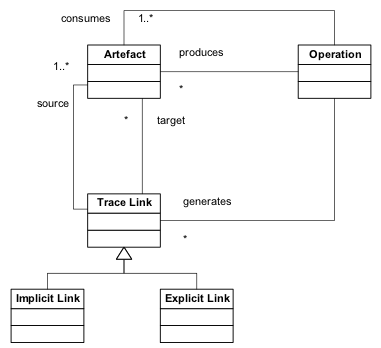
\includegraphics[scale=0.75]{./img/ExplicitImplicitTraceLinkClassification}
\caption{Clasificación de traceability inicial}
\label{fig:ClasifInicial}
\end{figure}

\subsection{Clasificación de enlaces de trazas implícita}

En la jerarquía de esta sección que se muestra en el dibujo \ref{fig:LinksImplicitos} se representan el conjunto de operaciones de \gls{mde} principales: consulta (Query Link), transformación (M2M Link), transformación modelo a texto (M2T Link), composición (Composition Link), actualización (Update Link), creación (Creation Link), eliminación (Delete Link), entre otras.


\begin{figure}[hbtp]
\centering
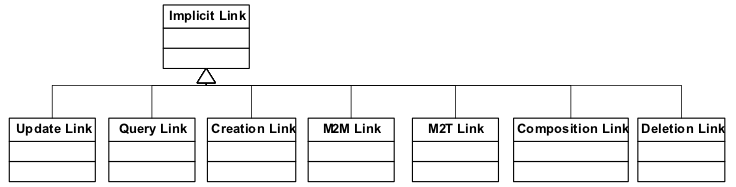
\includegraphics[scale=0.55]{./img/ImplicitTraceLinks}
\caption{Jerarquía de links implícitos}
\label{fig:LinksImplicitos}
\end{figure}


\subsection{Clasificación de enlaces de trazas explícitos}

En un principio esta clasificación se encuentra dividida en dos grandes grupos representados por las siguientes clases básicas: links modelo-modelo (por ejemplo las relaciones de dependencias \gls{uml}) y links modelo-artefacto (por ejemplo el enlace entre un modelo y un documento de texto que dicta un requerimiento), en el dibujo \ref{fig:LinksExplicitos} aparecen como Model-Model Link y Model-Artefact Link respectivamente.

Model-Model Link se encuentra a su vez subdividido en links estáticos (Static Link) y dinámicos (Dynamic Link). Los primeros representan relaciones estructurales que no cambian con el tiempo, en cambio los segundos representan información de los modelos que si pueden llegar a variar.

Los links estáticos pueden ser, o links consistentes (Consistent-With) donde dos modelos deben mantenerse de acuerdo o consistentes entre si, o links de dependencias (Dependency) donde la estructura y/o la semántica de un modelo depende de otro. Por su parte, los links de dependencia pueden ser: links de relación de subtipo (Is-A), links de referencias, links de subconjuntos, de importación y exportación, de uso, de refinamiento (Refines), etcétera.

Entre los links dinámicos se incluyen los links de llamadas (Calls) donde un modelo hace uso de métodos provisto por otro, los links de notificación (Notifies) donde es necesario almacenar información que puede ser manejada automáticamente. También las relaciones en tiempo de diseño como los links de generación o construcción (Generates), que indican qué información de un modelo es usada para producir o deducir otro, y las relaciones de sincronización (Synchronized With), donde el comportamiento de un conjunto de modelos se realiza de forma sincronizada.

El alcance de Model-Artefact Link es muy amplio, por tal motivo es esta clasificación solo se resumen un subconjunto de ejemplos, entre ellos: la relación satisface (Satisfies), que indica qué propiedad o requerimiento de un artefacto es satisfecha por un modelo; los links de asignación (Allocated-To), usados cuando la información de un artefacto no modelo es asignada a un modelo específico que la representa; la relación de realización (Performs), que indica qué tarea descripta por un artefacto es llevada a cabo por el modelo; las relaciones explica y respalda (Explains y Supports respectivamente) que dictan qué modelo se encuentra explicado/respaldado por un artefacto no modelo.

\begin{figure}[hbtp]
\centering
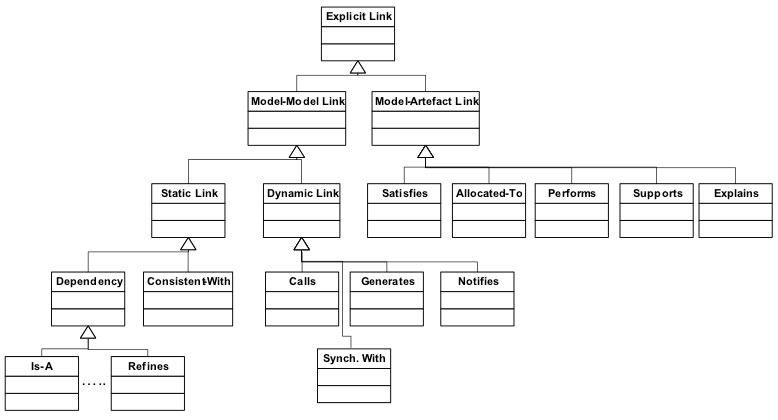
\includegraphics[scale=0.51]{./img/ExplicitTraceLinks}
\caption{Jerarquía de links explícitos}
\label{fig:LinksExplicitos}
\end{figure}



%%%%%%%%%%%%%%%%%%%%%%%%%%%%%
%%%% Propuesta %%%%%
%%%%%%%%%%%%%%%%%%%%%%%%%%%%%
\chapter{Manos a la obra}
\label{cap:Propuesta}

En este capítulo se introduce, desarrolla y fundamenta el esquema de traceability propuesto en la presente tesis.


\section{Esquema de traceability}


\subsection{Introducción}
\label{sec:EsquemaPropIntro}

La idea fundamental es lograr un meta-modelo bien simple en el que se capture solamente las ideas más relevantes de traceability y se almacene la información mínima necesaria. Gracias a todo lo anterior, y solo así, logramos obtener el concepto deseable de independencia del modelo con respecto al dominio en el que se quiera utilizar la funcionalidad de traceability. Concepto necesario para poder llegar a definir un esquema de propósito general que apunte principalmente a dar solución a los siguientes desafíos:

\begin{itemize}

\item Lograr un esquema que represente todas las trazas independientemente de como fueron generadas, si de forma explícita o implícitas, su granularidad y semántica.

\item Mantener la comunicación lo más simple posible, tanto la que existe entre los distintos usuarios en sus respectivos roles como la de los distintos tipos de herramientas que necesiten traceability.

\item La adaptación de una herramienta tiene que ser una tarea sencilla, cualquiera sea cuando desee agregar la funcionalidad de traceability mediante el uso de este esquema.

\item Aún dada la infinidad de artefactos que se pueden presentar, el esquema siempre tiene que ofrecer información semántica de los mismos, con el fin de facilitar la validación de enlaces legítimos.

\item Lograr identificar unívocamente cada artefacto sobre el que se desee realizar traceability.

\end{itemize}

\section{El esquema de traceability}

Con el fin de lograr respetar todas las consignas fundamentales listadas en \ref{sec:EsquemaPropIntro}, se definió una propuesta de un esquema de traceability que se encuentra representado mediante un diagrama de clases que se puede observar en el dibujo \ref{fig:EsquenaPropuesto}.

Como se puede observar, el meta-modelo se puede dividir lógicamente en dos partes principales, la primordial en la que se encuentran las abstracciones fundamentales de los elementos mínimos necesarios en cualquier herramienta que desee ofrecer traceability, y una secundaria en la que se engloba la configuración del esquema. Esta configuración permite ofrecer un meta-modelo flexible a cualquier escenario/dominio en el que se desee hacer uso de traceability.


\begin{figure}[hbtp]
\centering
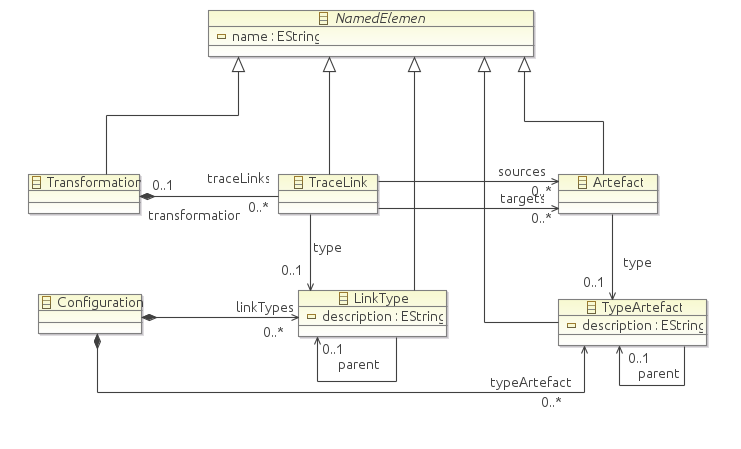
\includegraphics[scale=0.75]{./img/Esquema}
\caption{Esquema de traceability propuesto}
\label{fig:EsquenaPropuesto}
\end{figure}


\subsubsection{Clases fundamentales}

Entre los elementos fundamentales se encuentra la clase TraceLink, la cual representa una traza. Esta clase está compuesta por un nombre que sirve como identificador (name), un tipo con el cual se determina su semántica (type), una referencia de la transformación a la que pertenece la cual es optativa porque una traza puede o no ser producto de una transformación, y por último dos conjuntos de artefactos: el de los orígenes/fuentes (sources) y el de los objetivos/resultados (targets).

Los artefactos se encuentran representados por la clase Artefact, cuya identificación también pasa por su nombre (name), su descripción también por un diccionario de clave-valor, y por último su semántica también puede ser definida por un tipo definido en la configuración.

Por último entre los elementos fundamentales, tenemos la clase Transformation que abstrae de las transformaciones un nombre para su identificación, una descripción vía un diccionario y la colección de TraceLinks que son producto de su ejecución.


\subsubsection{Configuración del esquema}

Esta parte refleja la configuración necesaria para lograr un esquema adaptable a la infinidad de escenarios en los que puede aplicarse el mismo. Dicha configuración consiste en la definición de dos jerarquías, una que define la semántica de los artefactos que se van a tracear, y la otra para determinar la semántica de las trazas que pueden llegar a crearse. Ambas jerarquías están determinadas mediante las clases LinkType y TypeArtefact respectivamente, éstas comparten la siguiente estructura: un nombre (name) que las identifica, un texto que posibilita describirlas (description) y una relación (parent) que asocia una clasificación con su padre, gracias a dicha relación se logra la estructura jerárquica.

Un ejemplo de una configuración de tipos de trazas puede ser la jerarquía propuesta en la sección \ref{sec:ClasificacionTraceability}, que se puede ver siguiendo los diagramas \ref{fig:ClasifInicial}, \ref{fig:LinksImplicitos} y \ref{fig:LinksExplicitos}.


\subsection{Lo que no ofrece}

A continuación se lista un conjunto de aspectos y/o funcionalidades que el esquema propuesto actual no ofrece o tiene en cuenta:

\begin{itemize}

\item funcionalidad de versionado: que permita navegar por las trazas y refleje las modificaciones conjunto con las que se fueron realizando sobre los artefactos relacionados en el tiempo, a lo largo de la evolución de todas las tareas que forman parte de la ingeniería de un software.

\item métodos de detección o información de errores: que determine o informe cuando una traza es inválida.

\end{itemize}


\section{El prototipo}

En la presente sección se explica y presenta el prototipo desarrollado como ejemplo de la idea de la herramienta de traceability propuesta en la tesis.

\subsection{¿Cuál es la idea?}

La idea es lograr una herramienta que dada una definición de una transformación conjunto con sus modelos de entrada para su ejecución y sus modelos resultados, retorne el mapa de trazas 


%%%%%%%%%%%%%%%%%%%%%%%%%%%%%
%%% tecnologías %%%%%
%%%%%%%%%%%%%%%%%%%%%%%%%%%%%
\chapter{Descripción de tecnologías}

En el presente capítulo se realiza una breve introducción sobre cada una de las tecnologías que fueron utilizadas para la implementación del prototipo que hace uso del esquema propuesto de traceability.


\section{Eclipse}

Empezamos con el proyecto base sobre el cual el prototipo va a funcionar/ejecutarse, en la presente sección daremos una introducción a Eclipse en la que se presenta el proyecto y se detalla en breve la plataforma con sus principales componentes y/o funcionalidades.


\subsection{El proyecto}

Según se presenta en \cite{EMFADG, Eclipse} Eclipse es un proyecto de desarrollo de software de código abierto, cuyo propósito es proveer una plataforma de herramientas altamente integradas para la construcción, implementación y administración de software a lo largo de todo su ciclo de vida.

El proyecto núcleo es un framework genérico para la integración de herramientas conjunto con un entorno de desarrollo Java que ya se incluye para usarlo. Otros proyectos extienden el framework núcleo para soportar distintos tipos de herramientas y ambientes de desarrollo específicos. Estos proyectos en Eclipse están implementados en Java y pueden ser ejecutados en muchos sistemas operativos.

La comunidad Eclipse tiene más de 200 proyectos, los cuales pueden conceptualmente organizarse dentro de las siguientes 7 categorías:

\begin{enumerate}

\item Enterprise Development

\item Embedded and Device Development

\item \gls{rcp}

\item \gls{ria}

\item Application Frameworks

\item \gls{alm}

\item \gls{soa}

\end{enumerate}

Eclipse hace uso de la \gls{epl}, dicha licencia comercial permite a las organizaciones incluir software Eclipse en sus productos comerciales, mientras que al mismo tiempo les solicita en retorno un aporte a la comunidad con algo del producto derivado comercializado.


\subsection{La plataforma Eclipse}
\label{subsec:PlatEclipse}

La plataforma Eclipse es un framework para la construcción de \glspl{ide}, el mismo ha sido descripto como ``un ambiente para cualquier cosa y nada en particular''. La plataforma define simplemente la estructura básica del \gls{ide}, luego mediante la definición de herramientas específicas que amplían y se conectan al framework terminan definiendo un \gls{ide} particular de forma colectiva.


\subsubsection{Arquitectura de plugins}

En Eclipse la unidad básica de funcionamiento, o sencillamente un componente, es llamado plugin-in. Tanto la plataforma misma de Eclipse como las herramientas que la extienden están compuestas por éstos plug-ins. Una herramienta sencilla puede consistir de un simple plug-in, pero las más complejas por lo general están divididas en varios de éstos.

Un plug-in incluye todo lo necesario para la ejecución del mismo, ésto puede ser: código Java, imágenes, textos, etc. También incluye un archivo manifiesto (plugin.xml), en el que se declaran las interconexiones con otros plug-ins.

Durante el arranque la plataforma Eclipse descubre todos los plug-ins disponibles, sin embargo éstos son sólo activados cuando es necesaria su ejecución con el fin de no ralentizar el arranque.


\subsubsection{Workspace}

Las herramientas integradas en Eclipse trabajan con archivos y carpetas ordinarias, pero también disponen de una \gls{api} de alto nivel que define los siguientes componentes: recursos (resources), proyectos y un espacio de trabajo (workspace).

\paragraph{Resource} Un recurso es la representación que da Eclipse de un archivo y/o una carpeta, a los que provee de capacidades adicionales como detectores de cambios (change listeners), marcadores como las listas por hacer (to-do list) y/o mensajes de errores, y un registro de historia de cambios.

\paragraph{Project} Un proyecto es un recurso especial de tipo carpeta que es asignada por el usuario a una carpeta del sistema de archivos, es la que contiene todos los recursos del proyecto y la que define el tipo del mismo.

\paragraph{Workspace} El workspace es el espacio de trabajo o contenedor virtual en el que se encuentran todos los proyectos del usuario.


\subsubsection{Workbench}

El Workbench es la ventana principal que se le presenta al usuario cuando ejecuta la plataforma Eclipse, se encuentra implementada usando \gls{swt} y JFace. Esta ventana principal, que se puede apreciar en la imagen \ref{fig:EclipseWorkbench} está compuesta de vistas, editores y perspectivas.

\begin{figure}[hbtp]
\centering
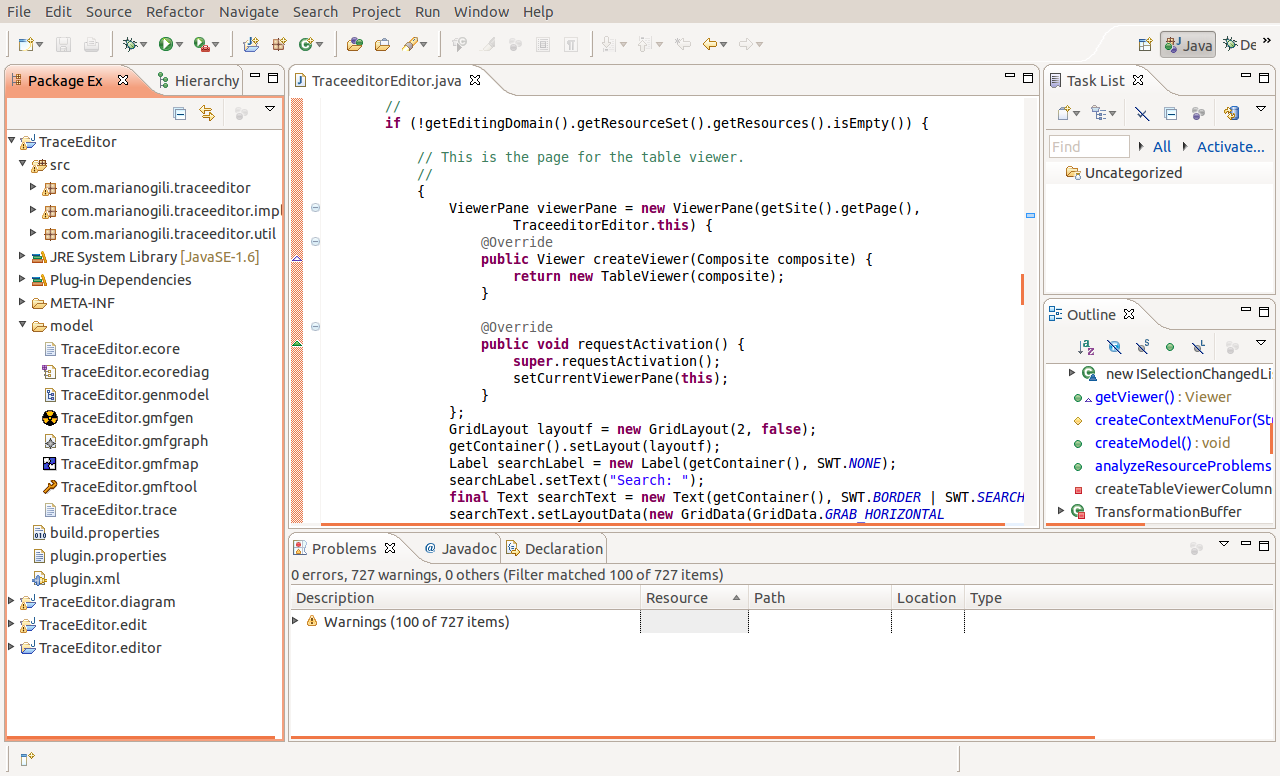
\includegraphics[scale=0.3]{./img/EclipseWorkbench}
\caption{Elcipse Workbench}
\label{fig:EclipseWorkbench}
\end{figure}

\paragraph{Editores} Éstos permiten al usuario abrir, editar y guardar distintos tipos de objectos.

\paragraph{Vistas} proveen información de algún objeto sobre el que el usuario se encuentra trabajando en el Workbench. Por ejemplo, una vista puede asistir un editor dando información sobre el documento que se está editando.

\paragraph{Perspectivas} Una perspectiva es sencillamente una agrupación de vistas y editores de manera que en su conjunto dan apoyo en una actividad completa.


\subsection{Resumen y más información}

Para cerrar y en resumen, la plataforma Eclipse proporciona un núcleo de elementos básicos y un conjunto de \glspl{api} genéricas, como el workspace y el workbench, y varios puntos de extensión a través del cual se pueden integrar nuevas funcionalidades. A través de estos puntos de extensión, las herramientas escritas como plug-ins independientes pueden extender la plataforma Eclipse.

Para obtener más información sobre el proyecto Eclipse ver \cite[\url{www.eclipse.org}]{Eclipse}, y para información técnica consultar \cite[Eclipse Platform Technical Overview]{EclipseTech}.


\section{Eclipse Modeling Framework}

A continuación proseguimos con una de las tecnologías del proyecto Eclipse usada para la implementación de una parte del prototipo, el framework \gls{emf} \cite{EMF}.

\subsection{El framework EMF}

El \gls{emf} es un framework de modelado y generación de código para herramientas de construcción y otras aplicaciones basadas en un modelo de datos estructurados. A partir de una especificación de un modelo descrito en \gls{xmi}, \gls{emf} provee herramientas y un entorno de ejecución para producir un conjunto de clases Java para el modelo y un conjunto de clases adaptadoras que permiten la visualización y la edición de dicho modelo.

\gls{emf} consiste de tres partes fundamentales:

\paragraph{EMF}

El framework \gls{emf} base incluye un meta-modelo (Ecore) para la descripción de modelos y soporte para un entorno de ejecución para dichos modelos que incluye las funcionalidades de notificación de cambios, persistencia por defecto vía serialización \gls{xmi} y una librería muy eficiente para la manipulación de objectos \gls{emf} genérica.

\paragraph{EMF.Edit}

El framework EMF.Edit incluye clases genéricas reusables para la construcción de editores de modelos \gls{emf}. Este provee:

\begin{itemize}

\item Clases proveedoras de contenido y etiquetas, acceso a propiedades orígenes y otras clases convenientes que permiten a los modelos \gls{emf} ser visualizados mediante entornos visuales estándares de escritorio (vía JFace) y/o hojas de propiedades.

\item Un framework de comandos que incluye un conjunto de clases que implementan comandos para la construcción de editores con soporte íntegro de deshacer y rehacer (undo/redo).

\end{itemize}

\paragraph{EMF.Codegen}

La funcionalidad de generación de código \gls{emf} es capaz de generar todo lo necesario para la construcción de un editor de un modelo \gls{emf} completo. Ésta incluye una \gls{gui} desde la cual las opciones de generación pueden ser especificadas y los generadores son invocados. Dicha funcionalidad de generación aprovecha el componente de Eclipse \gls{jdt}.

Tres niveles de generación de código son soportados:

\subparagraph{Model}

Proporciona la implementación de interfaces y clases Java para todas las clases del modelo, además la implementación de una clase fábrica y el paquete.

\subparagraph{Adapters}

Genera la implementación de las clases, llamadas ItemProviders, que se adaptan a las clases del modelo para su edición y visualización.

\subparagraph{Editor}

Produce un editor estructurado apropiadamente que se ajusta al estilo recomendado para los editores de modelo \gls{emf} de Eclipse y sirve como punto de partida para comenzar con la personalización.

\subsection{El (Meta) modelo Ecore}

Ecore es el modelo usado para representar modelos en \gls{emf}. Ecore es en sí mismo un modelo \gls{emf}, por lo cual es su propio meta-modelo. 

\begin{figure}[hbtp]
\centering
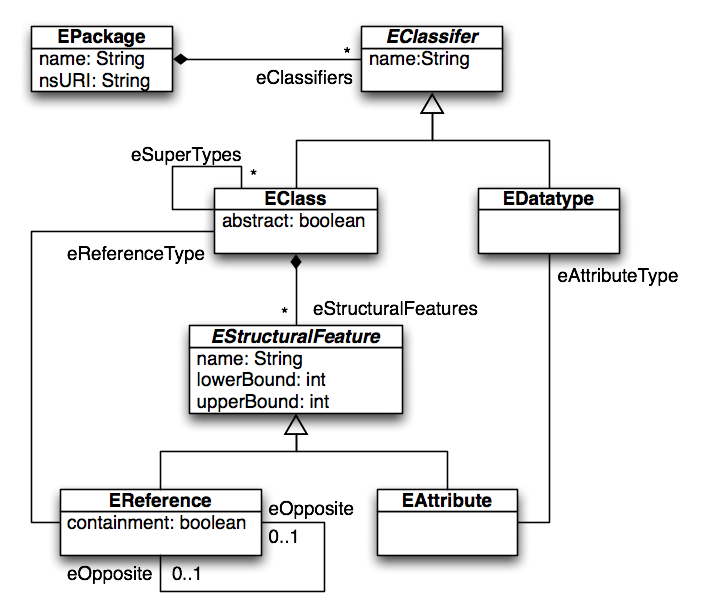
\includegraphics[scale=1]{./img/Ecore}
\caption{Modelo Ecore simplificado}
\label{fig:EcoreModel}
\end{figure}

Un modelo simplificado de Ecore se puede observar en la imagen \ref{fig:EcoreModel}, en particular lo conforman las siguientes cuatro clases Ecore principales:

\paragraph{EClass} Usada para representar una clase en el modelo. Tiene un nombre, atributos y referencias.

\paragraph{EAttribute} Para representar en el modelo un atributo. Tiene un nombre y un tipo.

\paragraph{EReference} Para representar una relación entre clases. Tiene un nombre, una marca que indica si es una composición, y el tipo de clase referenciada u objetivo que es otra clase.

\paragraph{EDataType} Representa el tipo de un atributo. El mismo puede ser un tipo primitivo (int, float) o un tipo objeto.


\subsection{Beneficios y más información}

Además de incrementar la productividad gracias a la generación automática de código, el uso del framework \gls{emf} provee otros beneficios: la notificación de cambios, una funcionalidad de persistencia (como la serialización \gls{xmi} entre otras), y una \gls{api} genérica reflexiva muy eficiente que sirve para la manipulación de objetos \gls{emf}. Sin embargo, uno de los beneficios más importantes de este framework es que \gls{emf} provee las bases para la interoperabilidad con otras herramientas y aplicaciones que se basan en él. 

Más información sobre el framework \gls{emf} se puede obtener en \cite{EMF} y \cite{EMFADG}.


\section{Graphical Modeling Framework}

En la presente sección analizamos el framework \gls{gmf}, el mismo fue usado para el desarrollo de la parte gráfica del editor de trazas del prototipo.

\subsection{El framework GMF}

\gls{gmf} es un framework para la construcción de editores gráficos de modelado para la plataforma Eclipse, por ejemplo editores \gls{uml}, ECore, de procesos de negocios, diagramas de flujo, etc. Este framework está compuesto por un componente de generación (GMF Tooling) y un entorno de ejecución (GMF Runtime) que ayudan en el desarrollo de editores gráficos que se basan en \gls{emf} y \gls{gef}.

\subparagraph{GMF Tooling} incluye por un lado editores para crear y/o modificar los modelos que describen los aspectos de notación, semántica y utilidad de un editor gráfico, y por otro, un generador que da como resultado la implementación del editor definido.

\subparagraph{GMF Runtime} Los plug-ins generados con GFM-Tooling dependen de este componente que es el entorno de ejecución sobre el que va a correr el editor.

\subsection{Arquitectura}

En el diagrama de componentes que podemos ver en la figura \ref{fig:GMFArquitectura} se muestran las dependencias existentes entre el editor gráfico generado, el entorno GMF Runtime, \gls{emf}, \gls{gef} y la plataforma Eclipse. Como se puede ver, el editor gráfico \gls{gmf} depende del componente \gls{gmf} runtime, y a su vez hace uso directo de \gls{emf}, \gls{gef} y la plataforma Eclipse.


\begin{figure}[hbtp]
\centering
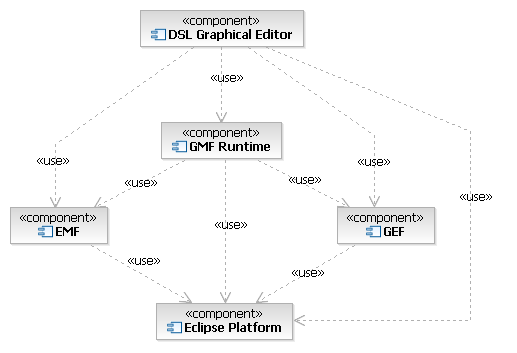
\includegraphics[scale=.75]{./img/GMFArquitectura}
\caption{Arquitectura GMF}
\label{fig:GMFArquitectura}
\end{figure}


\subsection{Modelos y flujo de trabajo}

En el diagrama \ref{fig:GMFWorkflow} se encuentran los principales componentes y modelos usados durante el desarrollo de un editor gráfico mediante el framework \gls{gmf}. Entre ellos se encuentra el concepto de \textbf{modelo de definición gráfica}, el cual contiene toda la información relacionada con los elementos gráficos que formarán parte del editor (figuras, nodos, enlaces, etc), pero que no tiene ninguna conexión directa o es dependiente con ninguno de los componentes del modelo de dominio para el cual ofrecerá la representación y/o edición. También tenemos el \textbf{modelo de definición de herramientas} que es opcional y usado para el diseño de la paleta, el menú y las barras de herramientas.

Tanto la definición gráfica como la de las herramientas pueden funcionar para modelos variados de dominios, éste es uno de los objetivos de \gls{gmf}, lograr que estas definiciones sean reusables para distintos dominios que se puedan presentar. Lo anterior se logra gracias al uso de un \textbf{modelo de asignación o mapeo}, que se encuentra separado y vincula las definiciones gráficas y las herramientas con los correspondientes modelos de dominios seleccionados.

Una vez fueron definidas los mapeos o asignaciones, \gls{gmf} dispone de un \textbf{modelo de generación} el cual posibilita la definición de los detalles para la implementación de la siguiente y última fase, la generación del editor.


\begin{figure}[hbtp]
\centering
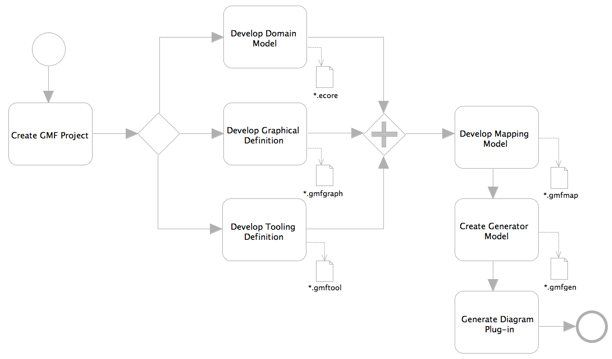
\includegraphics[scale=.65]{./img/GMFWorkflow}
\caption{Flujo de trabajo de GMF}
\label{fig:GMFWorkflow}
\end{figure}


\paragraph{Flujo de trabajo}

\begin{enumerate}


\item Creación del modelo del dominio, en este modelo se define la información no gráfica  que gestiona el editor.

\item Creación del modelo de definición gráfica, en el que se definen los elementos gráficos que se mostrarán/presentarán en el editor.

\item Creación del modelo de asignación gráfica, que es el que define la correspondencia entre los elementos del modelo del dominio con los elementos gráficos del modelo de definición gráfica.

\item Generación del editor gráfico.

\item Mejorar el editor gráfico por medio de la edición del código del plug-in generado.

\end{enumerate}


\subsection{Más información}

Más información sobre el framework \gls{gmf} se puede obtener en \cite{GMP}, \cite{IntroGMFRuntime} y \cite{GMFTutorial}.


\section{Atlas Transformation Language}

A continuación se da una introducción a la tecnología \gls{atl}, que no solo refiere a un lenguaje de transformación de modelos como su nombre puede confundir, sino que además trata de un conjunto de herramientas de desarrollo construidas para ser ejecutadas sobre la Plataforma Eclipse (introducida en \ref{subsec:PlatEclipse}).


\subsection{¿Qué es ATL?}

En el campo de \gls{mde}, \gls{atl} nos ofrece un medio para especificar la forma de producir un conjunto de modelos resultados/destinos a partir de un conjunto de modelos fuentes.

El lenguaje \gls{atl} es un híbrido de la programación declarativa e imperativa, dado que aunque el estilo declarativo es el más conveniente para la definición de las transformaciones, \gls{atl} también provee la posibilidad de construcciones imperativas con el fin de facilitar la especificación de algunos mapeos que en forma declarativa pueden llegar a resultar muy complejos de expresar.

Por otro lado, el \gls{ide} \gls{atl} provee un conjunto de herramientas estándar con el fin de facilitar el desarrollo de las transformaciones mediante este lenguaje como el  resaltado de sintaxis, el auto-completado de código, un depurador, entre otras.



\subsection{Conceptos de ATL}

Un modelo fuente se transforma en un modelo destino gracias a la definición de una transformación escrita en \gls{atl}, la cual también es un modelo. Los modelos fuente, destino y la definición de la transformación, cada uno conforman a sus respectivos meta-modelos y, a su vez, todos los meta-modelos se ajustan a \gls{mof} o Ecore. Esta relación se puede observar en la imagen \ref{ATL-concepts}.

Una transformación \gls{atl} es unidireccional, o sea que trabaja sobre un modelo fuente de solo lectura y produce un modelo destino de solo escritura. Durante la ejecución de una transformación, el modelo fuente puede ser navegado pero no cambiado, en cambio el modelo destino no puede ser navegado.

\begin{figure}[hbtp]
\centering
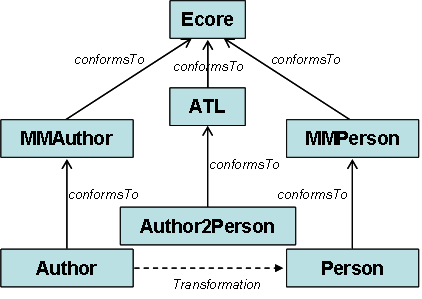
\includegraphics[scale=.65]{./img/ATL-concepts}
\caption{Modelos, transformaciones y sus meta-modelos}
\label{ATL-concepts}
\end{figure}


\subsection{El lenguaje ATL}

En este lenguaje de transformaciones modelo a modelo o \gls{mmt}, las operaciones de transformación son especificadas mediante módulos \gls{atl}. Cada módulo \gls{atl} permite a un desarrollador especificar la forma de producir un conjunto de modelos resultados desde un conjunto de modelos fuentes/orígenes. 

Además de módulos, este lenguaje permite crear programas que transforman modelos en tipos de datos primitivos (como booleanos, enteros o cadenas), lo cual se logra mediante la especificación de unidades llamadas \gls{atl} queries.

Por último \gls{atl} ofrece la posibilidad de desarrollar librerías independientes que pueden ser importadas a lo largo de diferentes tipos de unidades \glspl{atl}. Ésto nos da una forma conveniente de factorizar el código que va a ser usado por muchas unidades \gls{atl}.


\subsection{Más información}

Más información sobre la tecnología \gls{atl} se puede encontrar en la sección de documentación de la página del proyecto \cite[\url{www.eclipse.org/atl/}]{ATL}.


\section{QVT}

Por último en este capítulo dedicado a las tecnologías que forman parte de la presente tesis, se introduce el estándar para transformaciones especificado por la \gls{omg}, el lenguaje \gls{qvt}.


\subsection{Introducción a QVT}

\gls{qvt} como ya se dijo antes es el estándar de \gls{omg} para la definición de transformaciones. La especificación de \gls{qvt} es híbrida, como en el caso de \gls{atl}, relacional (o declarativa) y operacional (o imperativa). Comprende tres diferentes lenguajes \gls{mmt}: dos lenguajes declarativos llamados Relations y Core, y un tercer lenguaje, de naturaleza imperativa, llamado Operational Mappings. Puede observarse la relación de los meta-modelos de cada uno de los lenguajes en la figura \ref{QVTmetamodelos}. 

La naturaleza híbrida de este estándar fue introducida para abarcar distintos tipos de usuarios con diferentes necesidades, requisitos y hábitos.


\begin{figure}[hbtp]
\centering
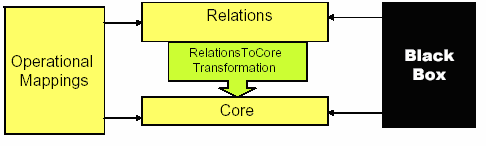
\includegraphics[scale=.65]{./img/metamodelosQVT}
\caption{Relación entre los meta-modelos QVT}
\label{QVTmetamodelos}
\end{figure}


\subsection{Lenguajes QVT}


\subsubsection{QVT declarativo}


\paragraph{Relations}

Es un lenguaje amigable para el usuario, que soporta pattern matching complejo y la creación de templates para objetos. Tiene creación de trazas implícita. También incluye la propagación de cambios, ya que provee un mecanismo para identificar elementos del modelo destino. 

\paragraph{Core}

Es un lenguaje pequeño con un soporte de pattern matching acotado. Tiene traceability explícito y las trazas pueden crearse y borrarse como cualquier otro objeto. Es igual de poderoso semánticamente que el lenguaje Relations pero trabaja a un nivel más bajo de abstracción. Esta propuesta absolutamente minimal lleva a que el lenguaje Core sea usado como un “assembler” de los lenguajes de transformación.


\subsubsection{QVT imperativo}


\paragraph{Operational Mappings}

Este lenguaje se especificó como una forma estándar para proveer implementaciones imperativas de transformaciones unidireccionales. También como el lenguaje Relations, dispone de creación de trazas implícita sobre el mismo modelo de trazas.


\paragraph{Implementaciones Black-box}

Estas implementaciones de caja negra, permite escribir transformaciones en otro lenguaje distinto a \gls{qvt}. Una implementación de este tipo no tiene
relación explicita con el lenguaje Relations, aunque una caja negra podría implementar una Relation, la misma debe ser responsable de mantener las trazas entre los elementos relacionados.


\subsection{Más información}

Para obtener más información introductoria consultar \cite{DSDPM}. Para más detalles técnicos y ejemplos se puede leer el documento de especificación \gls{mof} Query/View/Transformation \cite{QVT}.




%%%%%%%%%%%%%%%%%%%%%%%%%%%%%
%%% Trabajos relacionados %%%
%%%%%%%%%%%%%%%%%%%%%%%%%%%%%
\chapter{Trabajos relacionados}

En este capítulo se realiza una breve introducción de un conjunto de trabajos que tienen alguna relación con el tema en cuestión de la presente tesis, encontrados a lo largo del aprendizaje y la investigación.

\section{Un motor de traceability de transformación de modelos en la Ingeniería de Software}

En \cite{AmarLeblancCoulette} se describe un motor de traceability al que llamaron ETraceTool, que funciona como un plug-in de Eclipse programado mediante el paradigma orientado a aspectos con el fin de mantener aislada la generación de las trazas del código que pertenece a la transformación. El mismo trabaja sobre transformaciones escritas en Java usando la \gls{api} \gls{emf} \cite{EMF}. A continuación se listan sus principales características:

\begin{itemize}
\item El código de generación de trazas no es intrusivo en el código de la transformación;
\item La generación de trazas tiene que ser activada explícitamente por el diseñador de la transformación;
\item Los modelos de las trazas se encuentran aislados de los modelos origen y destino que forman parte de la transformación;
\item Los modelos de las trazas pueden ser usados a diferentes niveles de granularidad.
\end{itemize}

\begin{figure}[hbtp]
\centering
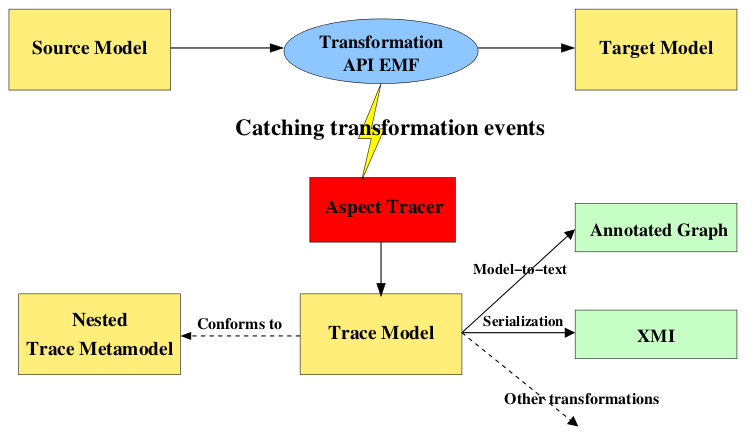
\includegraphics[scale=0.5]{./img/ETraceTool_Arquitectura}
\caption{Arquitectura de la herramienta ETraceTool}
\label{fig:ArqETraceTool}
\end{figure}

La arquitectura se puede apreciar en el dibujo \ref{fig:ArqETraceTool} y se explica de la siguiente manera, durante la transformación el plug-in captura un conjunto de eventos previamente identificados y clasificados gracias a la programación orientada a aspectos, luego el Aspect Tracer genera un modelo de trazas que conforma al meta-modelo de trazas anidado que se muestra en el dibujo \ref{fig:ETraceToolMeta-modelo}. Al final, el modelo de trazas generado puede ser serializado en un archivo \gls{xmi} o transformado a cualquier otro lenguaje mediante una transformación modelo-texto.

\begin{figure}[hbtp]
\centering
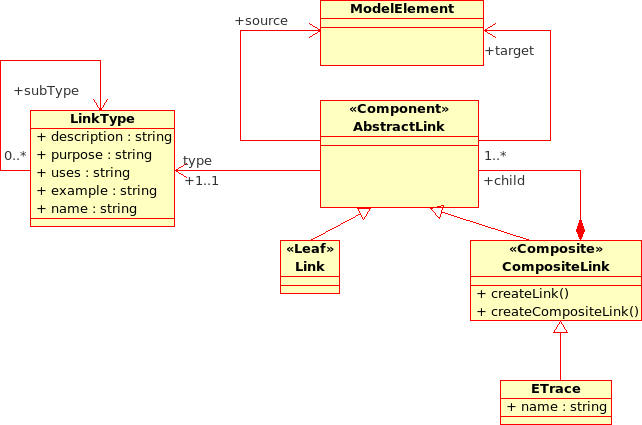
\includegraphics[scale=0.6]{./img/NestedTraceMetamodel}
\caption{Meta-modelo de trazas anidado}
\label{fig:ETraceToolMeta-modelo}
\end{figure}

El fundamento del diseño del meta-modelo de trazas anidado propuesto es para el caso en el que se presente una operación de transformación que llama o hace uso de otra transformación. En este caso el enlace compuesto permite separar las operaciones de bajo nivel (creación, eliminación, etc) de las operaciones de alto nivel (como una operación de refactorización).

\section{Un Framework de Traceability dirigido por modelos para el desarrollo de Software Product Line (SPL)}

El framework presentado en \cite{SousaKuleszaRummlerAnquetilMitschkeMoreiraAmaralAraujo} provee una plataforma abierta y flexible para crear enlaces de trazas entre distintos artefactos del desarrollo de una \gls{spl}. Pero, dado que el diseño del framework es genérico, éste también puede aplicarse o usarse en otras áreas del desarrollo \gls{spl}. El mismo ha sido diseñado e implementado basado en el uso de técnicas dirigidas por modelos. El meta-modelo de traceability descripto en el dibujo \ref{fig:SPLMeta-modelo} permite definir distintos tipos de enlaces de trazas entre los artefactos.

Las principales funcionalidades ofrecidas por el framework son las siguientes:

\begin{enumerate}
\item Creación y mantenimiento de los enlaces de trazas de artefactos existentes (modelos \gls{uml}, código fuente, etc);
\item Almacenamiento de los enlaces de trazas mediante el uso de un repositorio;
\item Búsqueda de enlaces de trazas específicos usando consultas de trazas predefinidas o personalizadas;
\item Visualización flexible de los resultados de las consultas de trazas por medio de diferentes tipos de vistas, como vista de árbol, grafo, tabla, etc.
\end{enumerate}

\begin{figure}[hbtp]
\centering
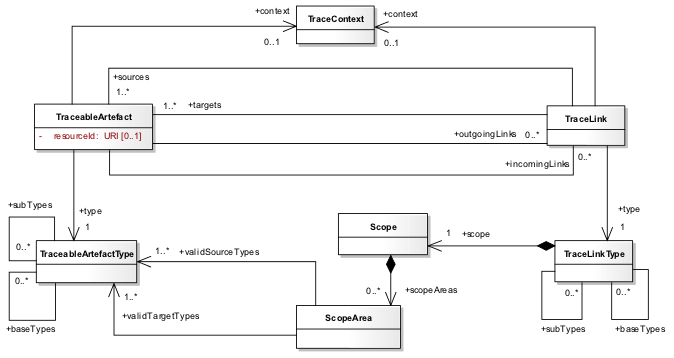
\includegraphics[scale=.6]{./img/Traceability_Metamodel}
\caption{Meta-modelo de traceability}
\label{fig:SPLMeta-modelo}
\end{figure}

\subsection{Meta-modelo de traceability}

Los elementos principales del meta-modelo son los siguientes:

\begin{itemize}
\item Un TraceableArtefact representa un artefacto que juega un rol en el ciclo del desarrollo. La granularidad del artefacto es arbitraria, puede ser un requerimiento, un diagrama \gls{uml}, un elemento de dicho diagrama, una clase o un método de dicha clase. El artefacto es identificado mediante la propiedad resourceId.
\item Un TraceLink es la abstracción de una transición de un artefacto a otro.
\item Cada TraceableArtefact tiene asignada una instancia de TraceableArtefactType, éstos se pueden encontrar agrupados de forma jerárquica.
 \item Análogo a los tipos de los artefactos los TraceLinks también tienen un tipo (TraceLinkType), teniendo en cuenta que la semántica de una relación entre dos artefactos puede variar.
\item Información adicional de artefactos y enlaces puede ser modelada mediante un contexto, el cual se encuentra representado por la clase TraceContext.
\item Las restricciones que determinan el conjunto de artefactos válidos, sobre los cuales los tipos de enlaces también son válidos se encuentran modeladas mediante los elementos ScopeArea y Scope.
\end{itemize}

\subsection{Arquitectura}

Como se muestra en el dibujo \ref{fig:SPLArquitectura}, la arquitectura ha sido definida en término de cuatro módulos principales. Cada uno de los cuales implementa una de las funcionalidades principales del framework, se detallan a continuación:

\begin{figure}[hbtp]
\centering
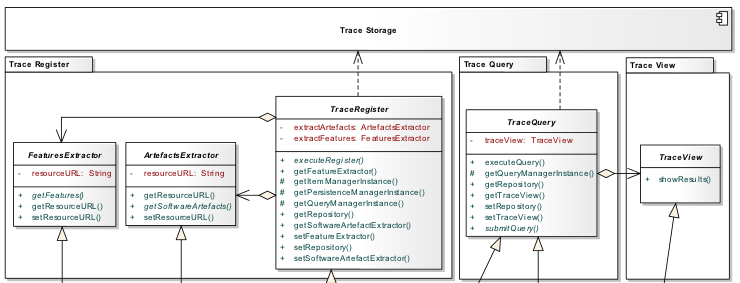
\includegraphics[scale=.55]{./img/ArquitecturaTraceabilityFramework}
\caption{Arquitectura del Framework de Traceability}
\label{fig:SPLArquitectura}
\end{figure}

\begin{enumerate}
\item Trace Register: este módulo provee mecanismos para crear y mantener (actualizar, eliminar y buscar) los enlaces de trazas;
\item Trace Storage: define los mecanismos de almacenamiento para persistir dichos enlaces;
\item Trace Query: este modulo permite crear y ejecutar consultas para buscar enlaces de trazas específicos que se encuentran previamente almacenados;
\item Trace View: usado específicamente para la representación visual de los enlaces resultados de una consulta realizada.
\end{enumerate}


\section{Integración de herramientas Case}

En \cite{KlarRoseSchurr} se presenta el problema real que sufre cualquier proceso de desarrollo actual, en el que como resultado del conjunto de actividades que lo conforman, se van generando una variedad muy amplia de artefactos de software (documentos de textos, hojas de cálculo, resultado de pruebas, modelos, gráficos, etc). Estos artefactos, aunque en esencia se encuentran relacionados lógicamente, al ser creados y manipulados por herramientas muy distintas que no fueron pensadas para interactuar (editores de textos, editores de modelo \gls{uml}, etc), las relaciones lógicas nombradas se pierden, o mejor dicho no existen o pasan desapercibidas en la práctica. En otras palabras, nos presenta el problema de la imposibilidad de traceability que encontramos entre la mayoría de las herramientas \gls{case} actuales.

Como solución a este problema, se propone un ambiente de integración para las herramientas \gls{case} al que llamaron TiE - Tool Integration Environment, el cual basa su integración en la creación de enlaces de trazas entre los artefactos de las distintas herramientas.

\section{Framework genérico de extracción de datos de traceability}

En \cite{GrammelKastenholz} proponen un framework genérico de traceability que toma como entrada una transformación de modelo y le aumenta arbitrariamente su funcionalidad con un mecanismo de traceability. En el dibujo \ref{fig:GenericoArquitectura} se muestra un panorama de alto nivel de la arquitectura propuesta. Ésta se basa en una interfase genérica que provee un punto de conexión para cualquier motor de transformación de modelos, mediante una \gls{api} que se ofrece al ingeniero que conecta su motor de transformación con el motor de traceability (oAW connector, \gls{qvt} connector). Como resultado el motor de transformación incluye la funcionalidad de traceability. El modelo de datos que usa el framework es el lenguaje específico de dominio para traceability al que llaman Trace-DSL.

\begin{figure}[hbtp]
\centering
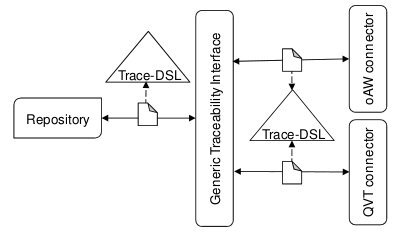
\includegraphics[scale=.7]{./img/GenericTraceFrame_Arquitectura}
\caption{Resumen de la arquitectura del Framework Genérico de Traceability}
\label{fig:GenericoArquitectura}
\end{figure}


Trace-DSL que se detalla en el dibujo \ref{fig:DSLTrace}, tiene como elemento raíz TraceModel. Artefact representa cualquier producto traceable generado durante el proceso de desarrollo, esto puede ser un requerimiento o una clase o un componente, como el método que pertenece a una clase. Todo artefacto es identificado unívocamente mediante un identificador único universal (UUID). TraceLink es una abstracción de una transición de un artefacto a otro dirigida por la relación desde-hacia entre artefactos origen y destino. TraceLink puede ser de uno de las siguientes cuatro instancias: CreateTraceLink, QueryTraceLink, UpdateTraceLink y DeleteTraceLink.


\begin{figure}[hbtp]
\centering
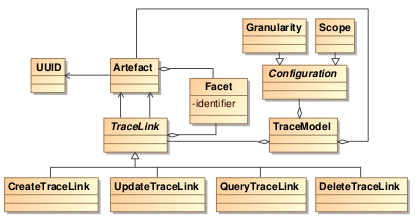
\includegraphics[scale=.8]{./img/Trace-DSL}
\caption{Lenguaje específico de dominio para traceability}
\label{fig:DSLTrace}
\end{figure}

Para la asignación de tipos a los artefactos y a los enlaces se usa el concepto de faceta, donde Trace-DSL asigna un conjunto de facetas (Facet) a cada uno de los mismos. Un ejemplo de faceta se da en el dibujo \ref{fig:FacetaCodigoFuente}. Además de lograr una solución simple al tipado de artefactos y enlaces, se obtiene un mecanismo fácilmente extensible y configurable al contexto donde se necesite aplicar traceability.

\begin{figure}[hbtp]
\centering
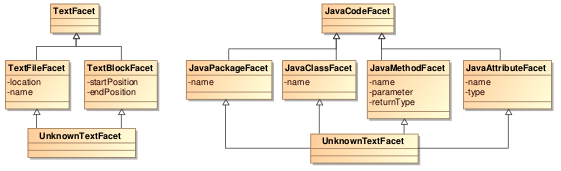
\includegraphics[scale=.72]{./img/Faceta}
\caption{Faceta para traceability de código fuente}
\label{fig:FacetaCodigoFuente}
\end{figure}

La configuración necesaria para hacer uso del framework implica:

\begin{enumerate}
\item Seleccionar las facetas requeridas para el escenario
\item Configurar la granularidad (Granularity) y el alcance (Scope)
\end{enumerate}

La configuración de la granularidad consiste en la especificación de qué tipos (definidos por las facetas) de artefactos y enlaces serán trazados para un escenario de traceability particular. En cambio la configuración del alcance implica restringir los datos de traceability a una combinación específica de valores. En otras palabras la primera solo chequea la existencia de facetas, mientras que la segunda adicionalmente examina las propiedades especificas de las facetas. Por ejemplo en el caso de TextFileFacet, puede ser necesario trazar solo archivos de textos con cierto nombre.

\section{Traceability local y global}

En la propuesta presentada en \cite{GlitiaEtienDumoulin} usan la idea de separación del proceso de traceability en los siguientes niveles, traceability en lo pequeño y traceability en lo grande refiriéndose a los mismos como traceability local y traceability global respectivamente.

\subsection{Meta-modelo de Traceability Local}

Este meta-modelo toma las trazas de la entrada y la salida de una única transformación. El meta-modelo está basado en el meta-modelo de trazas presentado en \cite{Jouault} y se muestra en el dibujo \ref{fig:LocalTraceMetamodel}.

\begin{figure}[hbtp]
\centering
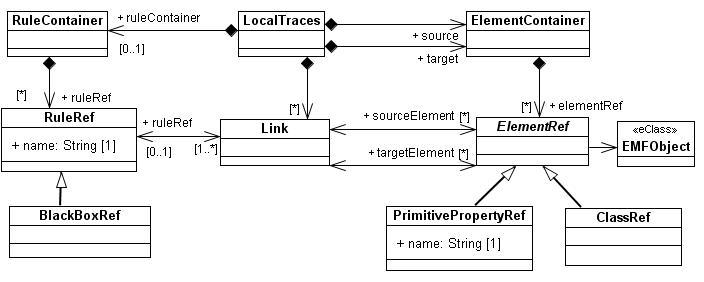
\includegraphics[scale=.55]{./img/LocalTraceMetamodel}
\caption{Meta-modelo de Trazas Local}
\label{fig:LocalTraceMetamodel}
\end{figure}

El meta-modelo de trazas local contiene dos conceptos principales Link y ElementRef en donde se expresa que uno o más elementos orígenes son enlazados a uno o más elementos objetivos. ElementRef es una clase abstracta que representa elementos que pueden ser traceados: instancias de clases o valores de propiedades. Los valores de las propiedades son traceados usando PrimitivePropertyRef el cual apunta a la instancia contenedora de la propiedad y tiene el nombre de la misma. Este tratamiento especial para los tipos primitivos de Java se debe a que no existen instancias de ellos en el modelo. Por otro lado las propiedades que son tipadas mediante una clase normal, son traceadas mediante ClassRef.

Para almacenar la información sobre las reglas de transformación aplicadas así como el caso particular de las cajas negras, se hace uso de los conceptos RuleRef y BlackBoxRef. En ambos casos, dado que pueden dar como resultado de su ejecución varios enlaces, se define la relación como uno a varios entre RuleRef y Link. RuleRef y BlackBoxRef son opcionales, en el caso de la primera solo se usa para realizar una depuración de las transformaciones, y la segunda si nos encontramos en la situación en la que ciertas partes del sistema no pueden ser pública su implementación.

ElementRef tiene una referencia al objeto real de los modelos origen y destinos. Como estos modelos están implementados mediante \gls{emf}, la referencia EMFObject es un EObject del meta-modelo Ecore. La clase LocalTraces representa la raiz del modelo de trazas local y tiene un RuleContainer que se usa como contenedor de las reglas y dos ElementContainer usados para agrupar los ElementRef origen y destino respectivamente. Separar los elemento orígenes y destinos permite reducir los costos de búsquedas de elementos de entrada o salida.

\subsection{Meta-modelo de Traceability Global}

Este meta-modelo enlaza trazas locales de acuerdo a la cadena que define la transformación. Un modelo de trazas global es el punto de entrada principal en el cual todas los modelos de trazas locales se encuentran, y describe qué modelo origen/objetivo de una transformación es el modelo objetivo/origen de la siguiente/previa transformación. En el dibujo \ref{fig:GlobalTraceMetamodel} se puede observar el meta-modelo.

\begin{figure}[hbtp]
\centering
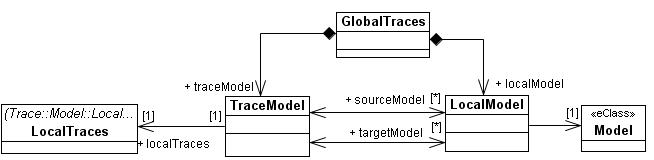
\includegraphics[scale=.6]{./img/GlobalTraceMetamodel}
\caption{Meta-modelo de Trazas Global}
\label{fig:GlobalTraceMetamodel}
\end{figure}

Este meta-modelo se engloban todas las trazas locales, los modelos de una cadena de transformación y la forma en que éstos se encuentran enlazados mediante TraceModel y LocalModel. Los modelos pueden ser compartidos entre distintas transformaciones, es decir uno puede ser producto de una transformación y también ser consumido por otra transformación.

Introducir este nivel global de trazas permite la navegación entre los modelos transformados y sus modelos de trazas locales, dando una mejor separación de lo que es en verdad la compleja información de traceability, lo que permite además una mejor flexibilidad para la creación de las trazas y la explotación de las mismas. No utilizar esta idea de trazas globales tiene como consecuencia disponer de todas las trazas en un único modelo de toda una cadena de transformación, lo cual desencadenaría en el colapso para la creación y la consulta de dicho modelo.

\subsection{¿Cómo trabaja el framework?}

Una de los principales objetivos de recolectar las trazas es dar luego la posibilidad a un usuario de inspeccionarlas realizando distintas consultas, una puede ser por ejemplo obtener los elementos relacionados a uno seleccionado. Este meta-modelo permite desde el modelo de trazas global navegar hacia los modelos de trazas locales y/o hacia a los modelos envueltos en cada una de las transformaciones. También desde el modelo de trazas local se puede navegar entre los elementos del modelo parte de la transformación.

En el dibujo \ref{fig:EjemploLocalGlobalMetamodel} se muestra un ejemplo de un modelo de trazas locales y globales producto de una cadena de transformación. En el ejemplo se representan los enlaces (Link) entre los elementos sin tener en cuenta las instancias de RuleRef para no sobrecargarlo.

\begin{figure}[hbtp]
\centering
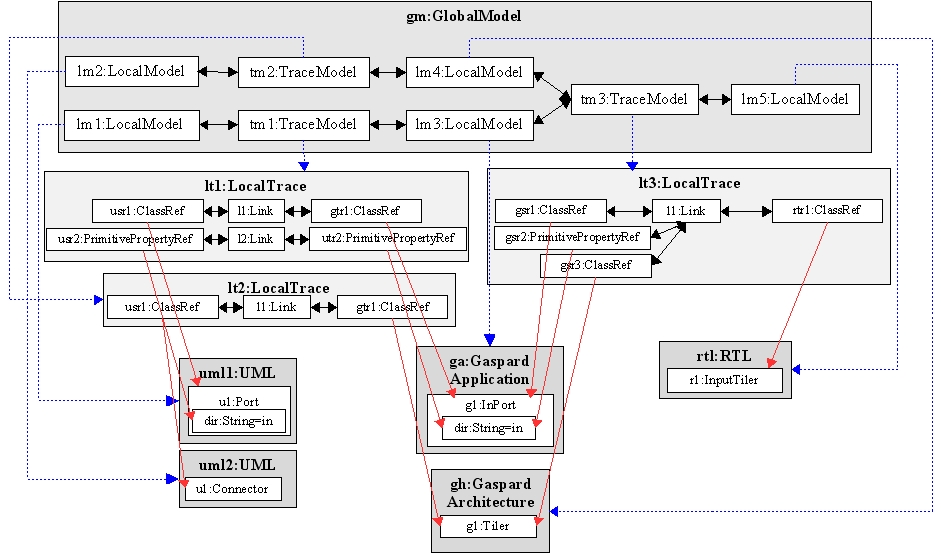
\includegraphics[scale=.45]{./img/EjemploLocalGlobalMetamodel}
\caption{Ejemplo de un modelo de trazas local y global}
\label{fig:EjemploLocalGlobalMetamodel}
\end{figure}


\backmatter

%%%%%%%%%%%%%%%%%%%%%%%%%%%%%
%%% Conclusión %%%%%
%%%%%%%%%%%%%%%%%%%%%%%%%%%%%
\chapter{Conclusión}


%%%%%%%%%%%%%%%%%%%%%%%%%%%%%
%%% Glosario %%%%%
%%%%%%%%%%%%%%%%%%%%%%%%%%%%%

\printglossaries

%%%%%%%%%%%%%%%%%%%%%%%%%%%%%
%%% Bibliografía %%%%%
%%%%%%%%%%%%%%%%%%%%%%%%%%%%%
\bibliographystyle{acm}
\begin{thebibliography}{99}


\bibitem{IEEE} IEEE Standard Glossary of Software Engineering Terminology. Number Std 610.12-1990, IEEE (1990).

\bibitem{BrcinaRiebisch} R. Brcina and M. Riebisch: Defining a Traceability Link Semantics for Design Decision Support. In: ECMDA Traceability Workshop (ECMDA-TW) 2008 Proceedings.

\bibitem{GrammelVoigt} B. Grammel and K. Voigt: Foundations for a Generic Traceability Framework in Model-Driven Software Engineering. In: ECMDA Traceability Workshop (ECMDA-TW) 2009 Proceedings.

\bibitem{Glossary} Glossary of Center of Excellence for Software Traceability (CoEST) \url{http://www.coest.org/index.php/traceability/glossary}.

\bibitem{Excellence} Center of Excellence for Traceability - Problem Statements and Grand Challenges. In: Center of Excellence of Traceability Technical Report (COET-GCT-06-01-0.9) September 10, 2006.

\bibitem{GotelFinkelstein} Gotel, O.C.Z., Finkelstein, A.C.W., “An Analysis of the Requirements Traceability Problem”, International Conference on Requirements Engineering, ICRE’94, Los Alamitos, California, Abril, 1994, pp 94-101.

\bibitem{DrivalosPaigeFernandesKolovos} N. Drivalos, R. F. Paige, K. J. Fernandes, D. S. Kolovos: Towards Rigorously Defined Model-to-Model Traceability. In: ECMDA Traceability Workshop (ECMDA-TW) 2008 Proceedings.

\bibitem{GlitiaEtienDumoulin} F. Glitia, A. Etien and C. Dumoulin: Fine Grained Traceability for an MDE Approach of Embedded System Conception. In: ECMDA Traceability Workshop (ECMDA-TW) 2008 Proceedings.

\bibitem{Jouault} F. Jouault: Loosely Coupled Traceability for ATL, In: Proceedings of the European Conference on MDA Traceability Workshop, Nurnberg, Germany (2005).

\bibitem{PaigeOlsenKolovosZschalerPower} R. Paige, G. Olsen, D. Kolovos, S. Zschaler, C. Power: Building Model-Driven Engineering Traceability Classifications, In: ECMDA Traceability Workshop (ECMDA-TW) 2008 Proceedings.

\bibitem{KlarRoseSchurr} F. Klar, S. Rose, A. Schurr: TiE - A Tool Integration Environment, In: ECMDA Traceability Workshop (ECMDA-TW) 2009 Proceedings.

\bibitem{AbidBotterweck} S. B. Abid, G. Botterweck: Resolving Product Derivation Tasks using Traceability in Software Product Lines, en: ECMDA Traceability Workshop (ECMDA-TW) 2009 Proceedings.

\bibitem{GrammelKastenholz} B. Grammel, S. Kastenholz: A Generic Traceability Framework for Facet-based Traceability Data Extraction in Model-driven Software Development, en: Proceedings of the 6\grad ECMFA Traceability Workshop (ECMFA-TW), 15 de junio de 2010, Paris, Francia.

\bibitem{AmarLeblancCoulette} B. Amar, H. Leblanc, B. Coulette: A Traceability Engine Dedicated to Model Transformation for Software Engineering. In: ECMDA Traceability Workshop (ECMDA-TW) 2008 Proceedings.

\bibitem{EMF} Eclipse Modeling Framework Project (EMF) \url{http://www.eclipse.org/modeling/emf/}.

\bibitem{SousaKuleszaRummlerAnquetilMitschkeMoreiraAmaralAraujo} A. Sousa, U. Kulesza, A. Rummler, N. Anquetil, R. Mitschke, A. Moreira, V. Amaral, J. Araújo: A Model-Driven Traceability Framework to Software Product Line Development. In: ECMDA Traceability Workshop (ECMDA-TW) 2008 Proceedings.

\bibitem{Eclipse} Eclipse Project \url{http://www.eclipse.org}.

\bibitem{EclipseTech} Eclipse Platform Technical Overview. Object Technology International, Inc., February 2003,
\url{http://www.eclipse.org/whitepapers/eclipse-overview.pdf}.

\bibitem{EMFADG} F. Budinsky, D. Steinberg, E. Merks, R. Ellersick, T. J. Grose: Eclipse Modeling Framework - A Developer's Guide. Addison Wesley.

\bibitem{GMP} Graphical Modeling Project \url{http://www.eclipse.org/modeling/gmp/}.

\bibitem{IntroGMFRuntime} Frederic Plante, IBM: Introducing the GMF Runtime, January 2006 \url{http://www.eclipse.org/articles/Article-Introducing-GMF/article.html}

\bibitem{GMFTutorial} Graphical Modeling Framework - Tutorial - Part 1 \url{http://wiki.eclipse.org/Graphical_Modeling_Framework/Tutorial/Part_1}

\bibitem{ATL} ATL Eclipse Project \url{http://www.eclipse.org/atl/}.

\bibitem{QVT} Meta Object Facility (MOF) 2.0 Query/View/Transformation Specification. Version 1.1, January 2011 - Version 1.0, April 2008. \url{http://www.omg.org/spec/QVT/index.htm}.

\bibitem{DSDPM} C. Pons, R. Giandini y G. Pérez: Desarrollo de Software Dirigido por Modelos. Conceptos teóricos y su aplicación práctica. Facultad de Informática, Universidad Nacional de La Plata. Octubre de 2008.


\end{thebibliography}


\end{document}
